
%% bare_conf.tex
%% V1.4b
%% 2015/08/26
%% by Michael Shell
%% See:
%% http://www.michaelshell.org/
%% for current contact information.
%%
%% This is a skeleton file demonstrating the use of IEEEtran.cls
%% (requires IEEEtran.cls version 1.8b or later) with an IEEE
%% conference paper.
%%
%% Support sites:
%% http://www.michaelshell.org/tex/ieeetran/
%% http://www.ctan.org/pkg/ieeetran
%% and
%% http://www.ieee.org/

%%*************************************************************************
%% Legal Notice:
%% This code is offered as-is without any warranty either expressed or
%% implied; without even the implied warranty of MERCHANTABILITY or
%% FITNESS FOR A PARTICULAR PURPOSE!
%% User assumes all risk.
%% In no event shall the IEEE or any contributor to this code be liable for
%% any damages or losses, including, but not limited to, incidental,
%% consequential, or any other damages, resulting from the use or misuse
%% of any information contained here.
%%
%% All comments are the opinions of their respective authors and are not
%% necessarily endorsed by the IEEE.
%%
%% This work is distributed under the LaTeX Project Public License (LPPL)
%% ( http://www.latex-project.org/ ) version 1.3, and may be freely used,
%% distributed and modified. A copy of the LPPL, version 1.3, is included
%% in the base LaTeX documentation of all distributions of LaTeX released
%% 2003/12/01 or later.
%% Retain all contribution notices and credits.
%% ** Modified files should be clearly indicated as such, including  **
%% ** renaming them and changing author support contact information. **
%%*************************************************************************


% *** Authors should verify (and, if needed, correct) their LaTeX system  ***
% *** with the testflow diagnostic prior to trusting their LaTeX platform ***
% *** with production work. The IEEE's font choices and paper sizes can   ***
% *** trigger bugs that do not appear when using other class files.       ***                          ***
% The testflow support page is at:
% http://www.michaelshell.org/tex/testflow/



\documentclass[conference]{IEEEtran}
% Some Computer Society conferences also require the compsoc mode option,
% but others use the standard conference format.
%
% If IEEEtran.cls has not been installed into the LaTeX system files,
% manually specify the path to it like:
% \documentclass[conference]{../sty/IEEEtran}





% Some very useful LaTeX packages include:
% (uncomment the ones you want to load)


% *** MISC UTILITY PACKAGES ***
%
%\usepackage{ifpdf}
% Heiko Oberdiek's ifpdf.sty is very useful if you need conditional
% compilation based on whether the output is pdf or dvi.
% usage:
% \ifpdf
%   % pdf code
% \else
%   % dvi code
% \fi
% The latest version of ifpdf.sty can be obtained from:
% http://www.ctan.org/pkg/ifpdf
% Also, note that IEEEtran.cls V1.7 and later provides a builtin
% \ifCLASSINFOpdf conditional that works the same way.
% When switching from latex to pdflatex and vice-versa, the compiler may
% have to be run twice to clear warning/error messages.






% *** CITATION PACKAGES ***
%
%\usepackage{cite}
% cite.sty was written by Donald Arseneau
% V1.6 and later of IEEEtran pre-defines the format of the cite.sty package
% \cite{} output to follow that of the IEEE. Loading the cite package will
% result in citation numbers being automatically sorted and properly
% "compressed/ranged". e.g., [1], [9], [2], [7], [5], [6] without using
% cite.sty will become [1], [2], [5]--[7], [9] using cite.sty. cite.sty's
% \cite will automatically add leading space, if needed. Use cite.sty's
% noadjust option (cite.sty V3.8 and later) if you want to turn this off
% such as if a citation ever needs to be enclosed in parenthesis.
% cite.sty is already installed on most LaTeX systems. Be sure and use
% version 5.0 (2009-03-20) and later if using hyperref.sty.
% The latest version can be obtained at:
% http://www.ctan.org/pkg/cite
% The documentation is contained in the cite.sty file itself.






% *** GRAPHICS RELATED PACKAGES ***
%
\ifCLASSINFOpdf
  % \usepackage[pdftex]{graphicx}
  % declare the path(s) where your graphic files are
  % \graphicspath{{../pdf/}{../jpeg/}}
  % and their extensions so you won't have to specify these with
  % every instance of \includegraphics
  % \DeclareGraphicsExtensions{.pdf,.jpeg,.png}
\else
  % or other class option (dvipsone, dvipdf, if not using dvips). graphicx
  % will default to the driver specified in the system graphics.cfg if no
  % driver is specified.
  % \usepackage[dvips]{graphicx}
  % declare the path(s) where your graphic files are
  % \graphicspath{{../eps/}}
  % and their extensions so you won't have to specify these with
  % every instance of \includegraphics
  % \DeclareGraphicsExtensions{.eps}
\fi
% graphicx was written by David Carlisle and Sebastian Rahtz. It is
% required if you want graphics, photos, etc. graphicx.sty is already
% installed on most LaTeX systems. The latest version and documentation
% can be obtained at:
% http://www.ctan.org/pkg/graphicx
% Another good source of documentation is "Using Imported Graphics in
% LaTeX2e" by Keith Reckdahl which can be found at:
% http://www.ctan.org/pkg/epslatex
%
% latex, and pdflatex in dvi mode, support graphics in encapsulated
% postscript (.eps) format. pdflatex in pdf mode supports graphics
% in .pdf, .jpeg, .png and .mps (metapost) formats. Users should ensure
% that all non-photo figures use a vector format (.eps, .pdf, .mps) and
% not a bitmapped formats (.jpeg, .png). The IEEE frowns on bitmapped formats
% which can result in "jaggedy"/blurry rendering of lines and letters as
% well as large increases in file sizes.
%
% You can find documentation about the pdfTeX application at:
% http://www.tug.org/applications/pdftex





% *** MATH PACKAGES ***
%
%\usepackage{amsmath}
% A popular package from the American Mathematical Society that provides
% many useful and powerful commands for dealing with mathematics.
%
% Note that the amsmath package sets \interdisplaylinepenalty to 10000
% thus preventing page breaks from occurring within multiline equations. Use:
%\interdisplaylinepenalty=2500
% after loading amsmath to restore such page breaks as IEEEtran.cls normally
% does. amsmath.sty is already installed on most LaTeX systems. The latest
% version and documentation can be obtained at:
% http://www.ctan.org/pkg/amsmath





% *** SPECIALIZED LIST PACKAGES ***
%
%\usepackage{algorithmic}
% algorithmic.sty was written by Peter Williams and Rogerio Brito.
% This package provides an algorithmic environment fo describing algorithms.
% You can use the algorithmic environment in-text or within a figure
% environment to provide for a floating algorithm. Do NOT use the algorithm
% floating environment provided by algorithm.sty (by the same authors) or
% algorithm2e.sty (by Christophe Fiorio) as the IEEE does not use dedicated
% algorithm float types and packages that provide these will not provide
% correct IEEE style captions. The latest version and documentation of
% algorithmic.sty can be obtained at:
% http://www.ctan.org/pkg/algorithms
% Also of interest may be the (relatively newer and more customizable)
% algorithmicx.sty package by Szasz Janos:
% http://www.ctan.org/pkg/algorithmicx




% *** ALIGNMENT PACKAGES ***
%
%\usepackage{array}
% Frank Mittelbach's and David Carlisle's array.sty patches and improves
% the standard LaTeX2e array and tabular environments to provide better
% appearance and additional user controls. As the default LaTeX2e table
% generation code is lacking to the point of almost being broken with
% respect to the quality of the end results, all users are strongly
% advised to use an enhanced (at the very least that provided by array.sty)
% set of table tools. array.sty is already installed on most systems. The
% latest version and documentation can be obtained at:
% http://www.ctan.org/pkg/array


% IEEEtran contains the IEEEeqnarray family of commands that can be used to
% generate multiline equations as well as matrices, tables, etc., of high
% quality.




% *** SUBFIGURE PACKAGES ***
%\ifCLASSOPTIONcompsoc
%  \usepackage[caption=false,font=normalsize,labelfont=sf,textfont=sf]{subfig}
%\else
%  \usepackage[caption=false,font=footnotesize]{subfig}
%\fi
% subfig.sty, written by Steven Douglas Cochran, is the modern replacement
% for subfigure.sty, the latter of which is no longer maintained and is
% incompatible with some LaTeX packages including fixltx2e. However,
% subfig.sty requires and automatically loads Axel Sommerfeldt's caption.sty
% which will override IEEEtran.cls' handling of captions and this will result
% in non-IEEE style figure/table captions. To prevent this problem, be sure
% and invoke subfig.sty's "caption=false" package option (available since
% subfig.sty version 1.3, 2005/06/28) as this is will preserve IEEEtran.cls
% handling of captions.
% Note that the Computer Society format requires a larger sans serif font
% than the serif footnote size font used in traditional IEEE formatting
% and thus the need to invoke different subfig.sty package options depending
% on whether compsoc mode has been enabled.
%
% The latest version and documentation of subfig.sty can be obtained at:
% http://www.ctan.org/pkg/subfig




% *** FLOAT PACKAGES ***
%
%\usepackage{fixltx2e}
% fixltx2e, the successor to the earlier fix2col.sty, was written by
% Frank Mittelbach and David Carlisle. This package corrects a few problems
% in the LaTeX2e kernel, the most notable of which is that in current
% LaTeX2e releases, the ordering of single and double column floats is not
% guaranteed to be preserved. Thus, an unpatched LaTeX2e can allow a
% single column figure to be placed prior to an earlier double column
% figure.
% Be aware that LaTeX2e kernels dated 2015 and later have fixltx2e.sty's
% corrections already built into the system in which case a warning will
% be issued if an attempt is made to load fixltx2e.sty as it is no longer
% needed.
% The latest version and documentation can be found at:
% http://www.ctan.org/pkg/fixltx2e


%\usepackage{stfloats}
% stfloats.sty was written by Sigitas Tolusis. This package gives LaTeX2e
% the ability to do double column floats at the bottom of the page as well
% as the top. (e.g., "\begin{figure*}[!b]" is not normally possible in
% LaTeX2e). It also provides a command:
%\fnbelowfloat
% to enable the placement of footnotes below bottom floats (the standard
% LaTeX2e kernel puts them above bottom floats). This is an invasive package
% which rewrites many portions of the LaTeX2e float routines. It may not work
% with other packages that modify the LaTeX2e float routines. The latest
% version and documentation can be obtained at:
% http://www.ctan.org/pkg/stfloats
% Do not use the stfloats baselinefloat ability as the IEEE does not allow
% \baselineskip to stretch. Authors submitting work to the IEEE should note
% that the IEEE rarely uses double column equations and that authors should try
% to avoid such use. Do not be tempted to use the cuted.sty or midfloat.sty
% packages (also by Sigitas Tolusis) as the IEEE does not format its papers in
% such ways.
% Do not attempt to use stfloats with fixltx2e as they are incompatible.
% Instead, use Morten Hogholm'a dblfloatfix which combines the features
% of both fixltx2e and stfloats:
%
% \usepackage{dblfloatfix}
% The latest version can be found at:
% http://www.ctan.org/pkg/dblfloatfix




% *** PDF, URL AND HYPERLINK PACKAGES ***
%
%\usepackage{url}
% url.sty was written by Donald Arseneau. It provides better support for
% handling and breaking URLs. url.sty is already installed on most LaTeX
% systems. The latest version and documentation can be obtained at:
% http://www.ctan.org/pkg/url
% Basically, \url{my_url_here}.




% *** Do not adjust lengths that control margins, column widths, etc. ***
% *** Do not use packages that alter fonts (such as pslatex).         ***
% There should be no need to do such things with IEEEtran.cls V1.6 and later.
% (Unless specifically asked to do so by the journal or conference you plan
% to submit to, of course. )


% correct bad hyphenation here
\hyphenation{op-tical net-works semi-conduc-tor}
\usepackage{graphicx}

\usepackage{booktabs}
\usepackage{subfig}
%\usepackage{subfigure}
\usepackage{lipsum}
\usepackage{array}
\usepackage{amsthm}
\usepackage{algorithm,amsmath}
\usepackage{algorithmic}
\usepackage{color,soul}
\usepackage{epstopdf}
\newcolumntype{L}[1]{>{\raggedright\let\newline\\\arraybackslash\hspace{0pt}}m{#1}}
\newcolumntype{C}[1]{>{\centering\let\newline\\\arraybackslash\hspace{0pt}}m{#1}}
\newcolumntype{R}[1]{>{\raggedleft\let\newline\\\arraybackslash\hspace{0pt}}m{#1}}
\renewcommand{\algorithmicrequire}{\textbf{Input:}}
\renewcommand{\algorithmicensure}{\textbf{Output:}}
\newcommand{\algorithmicbreak}{\textbf{break}}
\newtheorem{theorem}{Theorem}
\newtheorem{corollary}{Corollary}
\newtheorem{lemma}{Lemma}

\begin{document}
%
% paper title
% Titles are generally capitalized except for words such as a, an, and, as,
% at, but, by, for, in, nor, of, on, or, the, to and up, which are usually
% not capitalized unless they are the first or last word of the title.
% Linebreaks \\ can be used within to get better formatting as desired.
% Do not put math or special symbols in the title.
\title{Safe Multiclass Transfer Learning}


% author names and affiliations
% use a multiple column layout for up to three different
% affiliations
%\author{\IEEEauthorblockN{Michael Shell}
%\IEEEauthorblockA{School of Electrical and\\Computer Engineering\\
%Georgia Institute of Technology\\
%Atlanta, Georgia 30332--0250\\
%Email: http://www.michaelshell.org/contact.html}
%\and
%\IEEEauthorblockN{Homer Simpson}
%\IEEEauthorblockA{Twentieth Century Fox\\
%Springfield, USA\\
%Email: homer@thesimpsons.com}
%\and
%\IEEEauthorblockN{James Kirk\\ and Montgomery Scott}
%\IEEEauthorblockA{Starfleet Academy\\
%San Francisco, California 96678--2391\\
%Telephone: (800) 555--1212\\
%Fax: (888) 555--1212}}

% conference papers do not typically use \thanks and this command
% is locked out in conference mode. If really needed, such as for
% the acknowledgment of grants, issue a \IEEEoverridecommandlockouts
% after \documentclass

% for over three affiliations, or if they all won't fit within the width
% of the page, use this alternative format:
%
%\author{\IEEEauthorblockN{Michael Shell\IEEEauthorrefmark{1},
%Homer Simpson\IEEEauthorrefmark{2},
%James Kirk\IEEEauthorrefmark{3},
%Montgomery Scott\IEEEauthorrefmark{3} and
%Eldon Tyrell\IEEEauthorrefmark{4}}
%\IEEEauthorblockA{\IEEEauthorrefmark{1}School of Electrical and Computer Engineering\\
%Georgia Institute of Technology,
%Atlanta, Georgia 30332--0250\\ Email: see http://www.michaelshell.org/contact.html}
%\IEEEauthorblockA{\IEEEauthorrefmark{2}Twentieth Century Fox, Springfield, USA\\
%Email: homer@thesimpsons.com}
%\IEEEauthorblockA{\IEEEauthorrefmark{3}Starfleet Academy, San Francisco, California 96678-2391\\
%Telephone: (800) 555--1212, Fax: (888) 555--1212}
%\IEEEauthorblockA{\IEEEauthorrefmark{4}Tyrell Inc., 123 Replicant Street, Los Angeles, California 90210--4321}}




% use for special paper notices
%\IEEEspecialpapernotice{(Invited Paper)}




% make the title area
\maketitle

% As a general rule, do not put math, special symbols or citations
% in the abstract
\begin{abstract}
%In transfer learning, domain adaptation tries to exploit the knowledge from a source domain with a plentiful data to help learn a classifier for the target domain with a different distribution and little labeled training data. 
%Negative transfer could happen when the source and target domain are not related, especially for the multi-class scenario.
%In this paper, following the framework of \textit{Hypothesis Transfer Learning} (HTL), we propose a method that can safely transfer the knowledge from the source domain to the target and alleviate negative transfer using the LS-SVM in the multi-class scenario. Inspired by previous work, we propose a novel perspective on domain adaptation that can take an insight into the performance of transfer learning by data augmentation. We first augment data in the target domain by adding the auxiliary features using the outputs of the models trained from the source domain. We show that the performance of the target model is greatly affected by the weights (called transfer parameters) of the auxiliary features. To better estimate the transfer parameter, we propose a novel objective function to estimate the transfer parameters for the auxiliary features and alleviate negative transfer.
%Experiment results show that our method can alleviate negative transfer and outperform other transfer methods in the different scenario.


In transfer learning, domain adaptation tries to exploit the knowledge from a source domain with a plentiful data to help learn a classifier for the target domain with a different distribution and little labeled training data. 
In this paper, we investigate this problem under the setting of \textit{Hypothesis Transfer Learning} (HTL) where we can only access the source model instead of the data. In real world application, this scenario is common due to many reasons such as data credential.
As reported in \cite{ben2010theory}, negative transfer could happen when the source and target domains are not related, especially for the multi-class scenario. As we are not able to verify the source hypotheses in HTL, negative transfer could be an important issue.
In this paper, to study the problem of negative transfer in HTL, we propose a reformulation of HTL using the framework of Feature Augmentation (FA). Specifically, we first augment feature space of the target domain by adding the auxiliary features using the outputs of the models trained from the source domain. With this FA, we find the major theoretic reason that makes previous HTL work suffer from negative transfer, which is the in-proper selection of transfer parameter.
To better estimate the transfer parameter, we propose a novel objective function to learn a better transfer parameter.
Experiment results show that our method can alleviate negative transfer and outperform other transfer methods in the different scenarios.
\end{abstract}

% no keywords




% For peer review papers, you can put extra information on the cover
% page as needed:
% \ifCLASSOPTIONpeerreview
% \begin{center} \bfseries EDICS Category: 3-BBND \end{center}
% \fi
%
% For peerreview papers, this IEEEtran command inserts a page break and
% creates the second title. It will be ignored for other modes.
\IEEEpeerreviewmaketitle

\section{Introduction}
The success of transfer learning suggests that exploiting the knowledge of the existing models properly can greatly help us to learn new data. 
Transfer learning on image recognition is a very popular topic in recent years. Domain adaptation for image recognition tries to exploit the knowledge from a source domain with a plentiful data to help learn a classifier for the target domain with a different distribution and little labeled training data. In domain adaptation, the source and target domains share the same label but their data are drawn from the different distribution.

In domain adaptation, the knowledge of the source domain can be represented in 3 different approaches: instance, model and feature representation \cite{pan2010survey}. In this paper, we propose a method that transfers the knowledge from the source model. Some recent works show that exploiting the knowledge from the source model can boost the performance of the target model effectively, especially when there are just a few examples in the target data \cite{tommasi2014learning} \cite{fei2006one}.
Moreover, in some real applications, we can only obtain the source models and it is difficult to access their training data because of various of reasons such as the data credential.   
Recently, some works have been proposed within a framework called Hypothesis Transfer Learning (HTL) to handle this situation \cite{kuzborskij2013stability}. HTL assumes only source models (called the \textit{hypotheses}) trained on source task can be utilized and there is no access to source data, nor any knowledge about the relatedness of the source and target distributions. 
In HTL, a number of works have been attempted with Least Square Support Vector Machine (LS-SVM) \cite{kuzborskij2013stability}. Previous approaches show that the hypotheses can be evaluated effectively with LS-SVM via Leave-One-Out cross-validation \cite{tommasi2014learning}.

\begin{figure}[h]
\centering
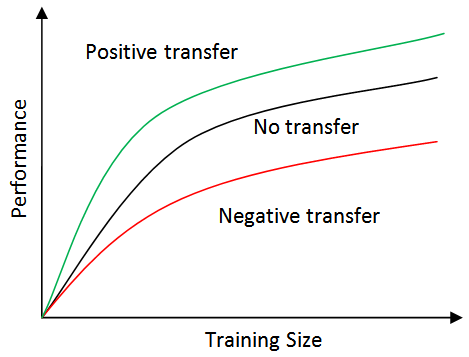
\includegraphics[scale=.5]{fig/negative.png}
\caption{Relying on the related source knowledge can improve the performance of the target model while forcing the target model to rely on the unrelated source could suffer from negative transfer.}
\end{figure}

In domain adaptation, different source domain can make the different contribution to the performance of the target model.
The theoretical research shows that the utility of the source domain decreases as the distributions of the source and target data become less similar (or \textit{less related})  \cite{ben2010theory} \cite{ben2007analysis}. Moreover, when the source and target tasks are not related, negative transfer may happen. In transfer learning, \textit{negative transfer} 
refers to the phenomenon where the source knowledge hurts the learning process and degrades the performance of the target model compare to a method without using any source knowledge \cite{pan2010survey}. 
Previous work of HTL assumes that the source and target domains are still very related. Most of them just consider the scenario where the target task is adding a new category to the source task (so called \textit{from N classes to N+1 classes}) \cite{tommasi2014learning} \cite{kuzborskij2013n} \cite{jie2011multiclass}. Moreover, their algorithms only focus on the performance on the newly added category, i.e. binary classification scenario, while paying less attention to the performance of the target model on all classes in the target data (the multi-class scenario). In some scenarios where the source and target tasks are less related, negative transfer could happen especially when we consider the performance of the target model on the whole target data (see Figure \ref{fig:distribution}).

%Previous works \cite{tommasi2014learning}, \cite{kuzborskij2013n} suggest that to better utilizing the hypotheses and reduce negative transfer, the decision of the algorithm should be made by combining the prior hypotheses and empirical knowledge (from the specific target task).

\begin{figure}
\centering
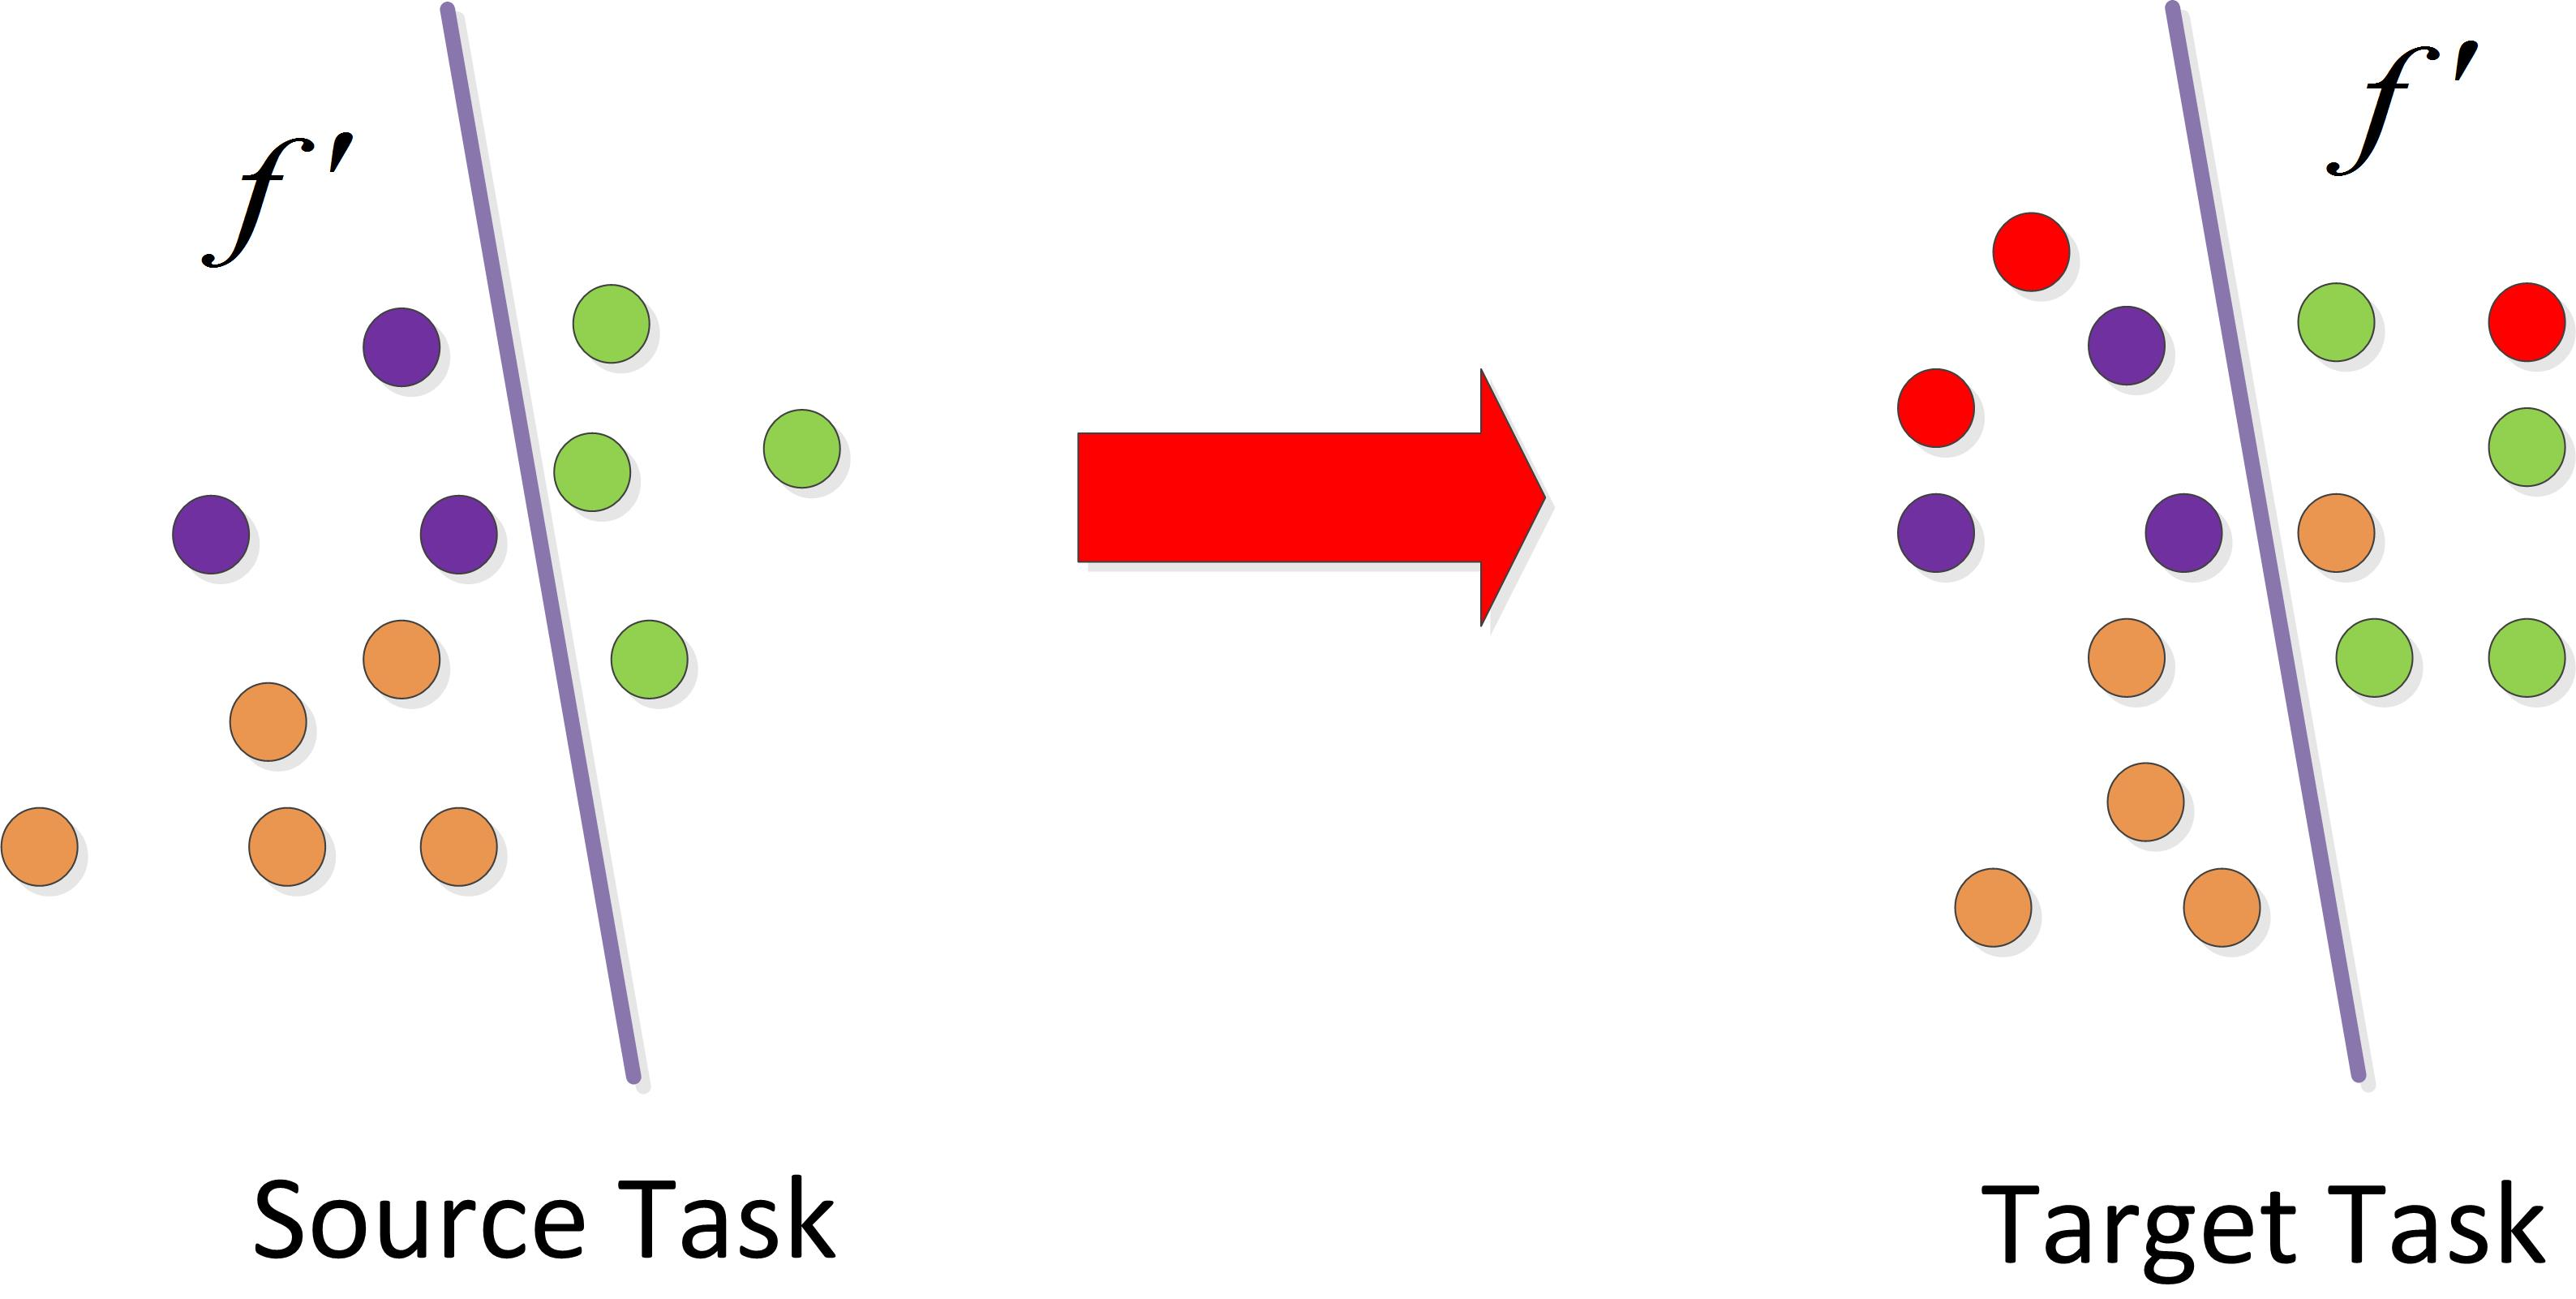
\includegraphics[scale=.5]{fig/domain.jpg}
\caption{Negative transfer happens when we transfer source hypothesis $f'$ to target one. Points with different color represent different categories. The data distribution would change when a new category is added into the dataset. The newly added category (red points) can also greatly affect the data distribution in target task and negative transfer could happen when we consider the multi-class scenario. }\label{fig:distribution}
\end{figure}

How to safely utilize the hypotheses to avoid negative transfer is still an open question in transfer learning \cite{Lu201514}. To avoid negative transfer, we have to evaluate the utilities of the hypothesis to keep useful knowledge and reject bad information. This approach can be achieved by setting different weights (called transfer parameters) to each hypothesis.
Previous works of HTL use Leave-One-Out error to estimate the transfer parameters and avoid negative transfer \cite{tommasi2014learning} \cite{kuzborskij2013n}. However, they try to solving a convex
optimization problem which minimizes an upper bound of
the leave-one-out error on the training set with a fix regularization term \footnote{In their original papers, this value is fixed to be 1. In our experiments, we found that this setting leads to degraded performance.}. As a result, when source and target domains are not related, previous methods suffer from negative transfer if this regularization term is not set properly (see experiments in Section \ref{sec:exp}).
In this paper, we propose our method, {called Safety Multiclass Transfer Learning (SMTLe)}, that can both alleviate negative transfer and leverage correct hypotheses to improve the performance of the target model. 
The main contributions of this paper include: (1) We propose a novel algorithm SMITLe within the HTL framework that can safely utilize the hypotheses to prevent negative transfer. We use a novel objective function with a L2 regularization term that can better estimate the transfer parameters and alleviate negative transfer. (2) We also show that by using sub-gradient descent, we can obtain the optimal solution at the rate of $O(\frac{\log(t)}{t})$ where $t$ is training iteration.
 
The framework of HTL with LS-SVM has two major phrases: (I) Building binary One-Versus-All SVMs with transfer parameters and biased regularization. (II) Estimating the transfer parameters with Leave-one-out error.
Following the two phrases of HTL, in Phrase I, inspired by the previous method, we reformulate the previous HTL problem as a data augmentation approach which reconstructs the target data by adding auxiliary features using the outputs of the source hypotheses. From the perspective of the data augmentation approach, we can turn our transfer learning problem into a traditional learning problem. We show that with proper values for the transfer parameter, we can always avoid negative transfer with our data augmentation approach. 
%We also show that it is necessary to add the regularization for the transfer parameter to get improved performance of the target model.
In Phrase II, 
based on the closed-form leave-one-out (LOO) error for model evaluation, we propose our novel objective function that can better estimate the transfer parameter and alleviate negative transfer with the L2 regularization term. We prove that transfer parameters learned from our novel objection function can alleviate negative transfer. Moreover, we show that we can always find a $\frac{\log(t)}{t}$ optimal solution with $t$ iterations using sub-gradient descent while previous methods are not able to get any guaranteed convergence rate.

In our experiment, initially, the data of the source and target domains are drawn from the same distribution (dataset). By adding the different level of the noise to the source data, we can generate several sources with different relatedness of the target domain. Experiment results show that when the source and target domain are related (no noise or very little noise is added), all the transfer methods can get improved result and our method outperforms the other baselines. As the source and target domain become less related, the baseline methods suffer from negative transfer while our method can still exploit knowledge from the source domain and the target model can get improved performance. 

The rest of this paper is organized as follow. In Section \ref{sec:work} we introduce the issues in transfer learning and some related work regarding these issues.
In Section \ref{sec:prob}, we introduce the biased regularization terms of our problem for Phrase I of HTL. Then, we propose a novel objective function for transfer parameter estimation, called SMTLe in Section \ref{sec:smitle}. We show that the estimated transfer parameter can evaluate the utility of the source hypothesis and avoid negative transfer autonomously. In Section \ref{sec:exp}, we show the performance comparison between SMTLe and other baselines on a variety of experiments on MNIST and USPS datasets.


\section{Related Work}\label{sec:work}
The motivation of transfer knowledge between different domains is to apply the previous information from the source domain to the target one, assuming that there exists certain relationship, explicit or implicit, between the feature space of these two domains \cite{pan2010survey}. Technically, previous work can be concluded into solving the following three issues: what, how and when to transfer \cite{tommasi2014learning}.


\textbf{What to transfer.} Previous work tried to answer this question from three different aspects: selecting transferable instances, learning transferable feature representations and transferable model parameters. Instance-based transfer learning assumes that part of the instances in the source domain could be re-used to benefit the learning for the target domain. Lim et al. proposed a method of augmenting the training data by borrowing data from other classes for object detection \cite{lim2012transfer}. Learning transferable features means to learn common feature that can alleviate the bias of data distribution in the target domain. Recently, Long et al. proposed a method that can learn transferable features with deep neural network and showed some impressive results on the  benchmarks \cite{LongICML15}. Model transfer
approach assumes that the parameters of the model for the source task can be transferred to the target task. Yang et al. proposed Adaptive SVMs by transferring parameters by incorporating the auxiliary classifier trained from source domain \cite{yang2007cross}. On top of Yang's work, Ayatar et al. proposed PMT-SVM that can determine the transfer regularizer according to the target data automatically \cite{aytar2011tabula}. Tommasi et al. proposed Multi-KT that can utilize the parameters from multiple source models for the target classes  \cite{tommasi2014learning}.
Kuzborskij et al. proposed a similar method to learn new categories by leveraging over the known source \cite{kuzborskij2013n}.

\textbf{When and how to transfer.} The question \textit{when to transfer} arises when we want to know if the information acquired from the previous task is relevant to the new one (i.e. in what situation, knowledge should not be transferred). 
\textit{How to transfer} the prior knowledge effectively should be carefully designed to prevent inefficient and negative transfer. Some previous work consists in using generative probabilistic method \cite{davis2009deep} \cite{wang2014active} \cite{zhou2014multi}.  Bayesian learning methods can predict the target domain by combining the prior source distribution to generate a posterior distribution. Alternatively, some previous max margin methods show that it is possible to learn from a few examples by minimizing the  Leave-One-Out (LOO) error for the training model \cite{kuzborskij2013n} \cite{tommasi2010safety}. Cawley et al. show that there is a closed-form implementation of LOO cross-validation that can generate unbiased model estimation for LS-SVM \cite{cawley2006leave}.

Our work corresponds to the context above. In this paper, we propose SMTLe based on model transfer approach with LS-SVM. We address our work on how to prevent negative transfer while just accessing the source model for domain adaptation. Compared to other works, propose a new perspective to the previous work of HTL, which brings more insight to negative transfer. Then we propose a novel strongly convex objective function for transfer parameters estimation. We show that SMTLe can converge at the rate of $O(\frac{\log(t)}{t})$. 
By optimizing this objective function, SMTLe can autonomously adjust the transfer parameters for different hypotheses. We theoretically show that, without any data distribution assumption, the superior bound of the training loss for SMTLe is the loss of a method learning directly (i.e. without using any prior knowledge). As a result, SMTLe can achieve a better performance and alleviate negative transfer.


\section{Transfer knowledge with feature augmentation}\label{sec:prob}
In this section, we focus on the Phrase I of HTL and introduce our biased regularization for binary LS-SVM for our problem. We propose a new perspective for transfer learning in HTL and analysis the reasons why negative transfer could happen.

\subsection{Feature augmentation in HTL}
We define our transfer task in the following way: Suppose we have $N$ visual categories. 
In our source task, $N$ source binary classifiers $f'_n(x)$ for $n=1,...,N$, are trained from a distribution $\mathcal{D}_s$ to distinguish whether an object belongs to each of the $N$ categories. In our target task, we have another small set of data $(x,y)$ drawn from another distribution $\mathcal{D}_t$ with the same $N$ categories as those in source task. We want to train $N$ target binary classifiers $f_n(x)$ for $n=1,...,N$ on the data of the target domain so that they can perform well on the target domain.

Vapnik et al. \cite{vapnik2015learning} proposed a diagram to transfer the privileged knowledge from the teacher to the student. The privileged knowledge is used as the auxiliary feature for training the student model. Inspired from this idea, we propose our feature augmentation approach for  HTL in domain adaptation. We treat the outputs of the source models as the auxiliary features and used them to train the target model. The difference between the auxiliary feature in our work and the privileged information is that we can use the auxiliary feature in both training and testing procedures while privileged knowledge can be used for training the model only.

\begin{figure*}
	\centering
	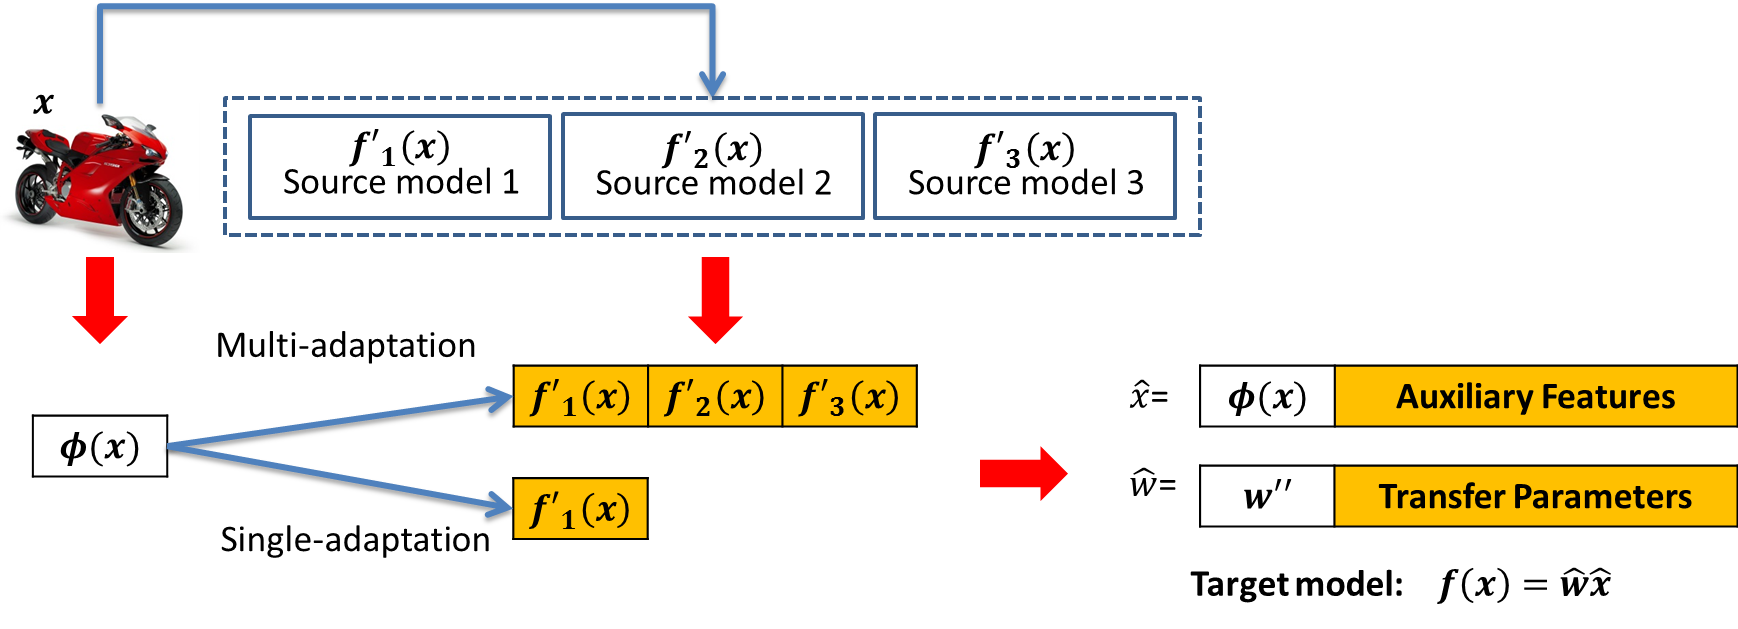
\includegraphics[scale=0.5]{fig/aug2.png}
	\caption{The transfer learning process can be considered as the augmentation of the target data where the decision scores of the source models are appended as the auxiliary features. The transfer parameters can be considered as the a part of the corresponding hyperplane. We can consider 2 augmentation strategies: multi-adaptation and single-adaptation.}\label{fig:aug}
\end{figure*}

As a result, when there are a group of $N$ source models $F'(x)=\{f'_i(x)|i=1,...,n\}$, we can augment the target feature space as  $\hat{x}=[\phi(x),f'_1(x),...,f'_N(x)]$ when we want to leverage the knowledge from multiple source models (Multi-adaptation) or $\hat{x}=[\phi(x),f'_r(x)], r\in 1,...,N$ (Single-adaptation). Here $\phi(x)$ can be any feature mapping that maps the example into another space. Thus the target binary model for category $n$ can be represented as $f_n=\hat{w}_n\hat{x}$, where $\hat{w}_n=[w_{n}'',\beta_1,...,\beta_N]$ (Multi-adaptation) or $[w_{n}'',\beta_r]$ (Single-adaptation). Here, we call the element(s) $\beta$ the \textit{Transfer Parameter}. 

\begin{equation}\label{eq:aug_pre}
\begin{aligned}
f_n(x)&=w_{n}''\phi(x)+\sum\limits_k^N{\beta _kw'_k\phi(x)}
\end{aligned}
\end{equation}
An intuitive interpretation of Eq. \eqref{eq:aug_pre} is that the auxiliary features can be considered as a similarity score from the source model. When the target model decides whether an object belongs to certain category, it also considers the decisions of the source model as the reference (the second part of the right hand side in Eq. \eqref{eq:aug_pre}).

$f_n$ can be formalized as the following optimization problem:
\begin{equation}\label{eq:svm_obj}
\begin{aligned}
\textbf{min} && \Omega(\hat{w}_n) + \frac{C}{2}\sum\limits_i^l {\mathcal{L}(f_n(x_i),Y_{in})} \\
\end{aligned}
\end{equation}
Here $\Omega({w})$ is the regularization term to guarantee good generalization performance and avoid overfitting. $Y_{in}$ is the encoded label for binary classifier following $Y_{in}=1$ if $y_i=n$ and $-1$ otherwise. $\mathcal{L}(\cdot)$ is the loss function. When we consider to use Least Square SVM as the classifier, we have $\mathcal{L}(f,y) = (f-y)^2$ and $\Omega({w}) = \frac{1}{2}||w||^2$. 

Compared to the previous methods in HTL, we have the following advantages:
\begin{itemize}
	\item Wider range selection of the source models. Most of the previous works in HTL are limited to their source models to the linear models \cite{tommasi2014learning} \cite{aytar2011tabula}. With the idea of feature augmentation, we can treat the source model as a whole which just outputs the decision score of an example. Therefore, we can exploit the knowledge of the different types, such as Neural Networks and inference models \footnote{Previous works, such as \cite{tommasi2014learning} \cite{aytar2011tabula}, can be considered as the special case of our problem where the linear model is used as the source. We can obtain similar objective function when we consider the transfer parameter as the hyper-parameter that can should be defined according to the background knowledge.}.
	\item Insight into the performance of the target model. By feature augmentation, we turn the HTL domain adaptation problem into a classical learning problem and we can better analysis some important problems existed in transfer learning such as negative transfer. In the next part, we introduce some analysis of how to improve the performance of the target model in our framework. 
\end{itemize}

\subsection{Reasons for negative transfer}
From the perspective of the feature augmentation, we can turn the problem of domain adaptation problem with HTL into a traditional learning problem, i.e. find the optimal values for the elements of the hyperplane hyperplane $\hat{w}=[w_{n}'',\beta_1,...,\beta_N]$ \footnote{We take Mult-adaptation for instance. The conclusion can be applied to Single-adaptation without any modification.}. According to the principle of Structural Risk Minimization (SRM) \cite{vapnik1999overview}, the risk of a linear classifier $f(x)=wx$ on the unseen test data $R(f)$ (generalization risk) is bounded by:
\begin{equation}\label{eq:srm}
R(f) \le {R_{emp}}(f) + \sqrt {\frac{{h(\ln (2l/h) + 1) + \ln (\delta /4)}}{l}} 
\end{equation}
Here the first part on the right-hand side of the inequation ${R_{emp}}(f)$ is the empirical risk (training error) of the classifier and the second part is the confidence interval. $h$ and $l$ denote the VC dimension and number of training data of the classifier respectively and $\delta$ is the confidential parameter. According to \cite{suykens1999least}, the VC dimension $h$ is bounded by $h \le \min([||w||^2R^2],l)+1$ where $R$ is the radius of the smallest ball containing data $x$ and $||w||$ is the \textit{2-norm} of the hyperplane.

As we discussed above, we use the outputs of the source models as the auxiliary features to augment the target data. Let $R$ and $\hat{R}$ denote the radius of the data before and after augmentation. We should have $R^2 \le \hat{R}^2$ and $||w||^2\le ||\hat{w}||^2$. This indicates that the VC dimension of the target model trained on the augmented data (augmented model) tends to increase compared to the model trained from the original data, i.e.  the method without transferring any source knowledge (no transfer model). As a result, feature augmentation eventually increases the confidence interval of the risk of the augmented model. When the augmented model failed to decrease the empirical risk, its performance would degrade, i.e. suffer from negative transfer. For example, when the auxiliary features can't provide any extra useful information for classification, i.e. the source domain and target domain are unrelated, negative transfer could happen. In contrast, if we can significantly decrease the empirical risk of the augmented model, we can decrease its generalization risk and get improved performance, i.e. positive transfer.

From the analysis above, we can see that in order to get improved performance and alleviate negative transfer, we have to carefully control the value of the transfer parameters. Following this idea, a simple method to estimate the hyperplane $\hat{w}$ for the target model solve optimizing problem \eqref{eq:svm_obj} directly. However, if we are not able to regularize the transfer parameters properly, the target model could easily suffer from negative transfer when the source and target are weakly related (see the experiment result for the method Feature+ in Section \ref{sec:exp}).
In next section, we introduce our method SMTLe to estimate the transfer parameters that can improve the performance of the target model and alleviate negative transfer .



\section{SMTLe}\label{sec:smitle}
In this section, we focus on the Phrase II of HTL, to estimate the transfer parameter in our task. We introduce an algorithm, called SMTLe, that can effectively estimate unbiased transfer parameter from a small training set and alleviate negative transfer. 

\subsection{Multiclass Prediction Loss with Leave-One-Out}
%\hl{In this part, we introduce our method to estimate the proper $\boldsymbol{\beta}$ that can prevent negative transfer. We use closed-form LOO error to evaluate the performance of SMTLe for multi-class classification.  and optimize $\boldsymbol{\beta}$ with our novel objective function to prevent negative transfer.}

In the previous section, we introduce a novel perspective for HTL and show that the Phrase I of HTL is equivalent to augmenting the target data with the outputs of the source models. We show that how to set the values of the transfer parameters can significantly affect the performance of the target model. We have to decrease the empirical risk to improve the performance and alleviate negative transfer. In this part, we introduce the multiclass Leave-One-Out cross-validation  (LOO-CV) error to estimate the empirical risk of the target model.

%From Phrase I, we can see that the amount of knowledge transferred is determined by the transfer parameter $\boldsymbol{\beta}$. Generally, we would like to reduce the amount of transfer from the source hypotheses when they are not related. Meanwhile, for those correct ones, aggressively increasing the amount of transfer can boost the performance of the target model. Once we fix the value of $\boldsymbol{\beta}$, our task can be solved directly.

As we discussed above, we have to choose the proper transfer parameters $\boldsymbol{\beta}$ to minimize the empirical risk on the target training set to exploit the source knowledge.
In this paper, we choose the Leave-One-Out (LOO) cross-validation error to estimate the empirical risk. We choose it for the following reasons: (1) It is proven that LOO error has a low bias on small training data regime \cite{kuzborskij2013stability}. (2) The Leave-One-Out error is an almost unbiased estimator of the generalization error \cite{elisseeff2003leave}. (3) Moreover, for LS-SVM, we can obtain unbiased LOO-CV error in closed form which means we can estimate the values of the transfer parameters in a more efficient way.

Let $K(X,X)$ be the kernel matrix and
\begin{equation}\label{eq:linear}
\psi=\left[ 
{K(X,X) + \frac{1}{C}{\rm{I}}} \right]
\end{equation}
The unbiased LOO estimation for sample $x_i$ can be written as \cite{cawley2006leave}:
\begin{equation} \label{eq:loo}
{\hat Y_{in}} = {Y_{in}} - \frac{{{\alpha _{in}}}}{{\psi_{ii}^{ - 1}}}\quad {\text{for}}\quad n = 1,...,N
\end{equation}
Here $\psi^{-1}$ is the inverse of matrix $\psi$ and  $\psi_{ii}^{-1}$ is the $ith$ diagonal element of $\psi^{-1}$. 

Let $F'(X)=\left[f'_1(X),...,f'_N(X)\right]$ be the output matrix of the source models and define $\begin{array}{c}\boldsymbol{\alpha'} \end{array}$ and $\begin{array}{c}\boldsymbol{\alpha}''\end{array}$ as follow:
\begin{equation}
\begin{array}{cc}
\boldsymbol{\alpha'} =\psi^{-1} \times Y & \boldsymbol{\alpha''} =\psi^{-1} \times F'(X)
\end{array}
\end{equation}

The matrix $\boldsymbol{\alpha}=\{\alpha_{in}\}$ in Eq. \eqref{eq:loo} can be calculated as:
\begin{equation}\label{eq:solution}
 \boldsymbol{\alpha}  = \boldsymbol{\alpha} ' - \boldsymbol{\alpha} ''\boldsymbol{\beta ^T}
\end{equation}

Let us call $\xi_i$ the multi-class prediction error for example $x_i$. $\xi_i$ can be defined as \cite{crammer2002algorithmic}:
\begin{equation}\label{eq:train_loss}
\xi_i(\beta) = \mathop {\max }\limits_{n \in \left\lbrace 1,...,N \right\rbrace } {\left[ {1 - {\varepsilon _{n{y_i}}} + {{\hat Y}_{in}}\left( {\beta_n } \right) - {{\hat Y}_{i{y_i}}}\left( {\beta_{y_i} } \right)} \right]}
\end{equation}
Where $\varepsilon _{n{y_i}}=1$ if $n=y_i$ and 0 otherwise. The intuition behind this loss function is to enforce the distance between the true class and other classes to be at least 1. 



Now, we already have an effective way to measure the performance of the target model with different $\boldsymbol{\beta}$ for our task. In the next part, we introduce how we optimize the parameters.
\subsection{Loss Function of SMTLe}
In this part, we propose a novel objective function according to our multi-class prediction loss function for transfer parameter estimation. We show that we can effectively obtain the optimal  $\boldsymbol{\beta}$ that is resistant to negative transfer. 
 
From Eq. \eqref{eq:train_loss} we can see that, different from the binary scenario where 0 is used as the hard threshold to distinguish the two classes, our multi-class loss only depends on the gap between the decision function value of the correct label ($\hat Y_{y_i}$) and the maximum among the decision function value of the other labels ${{\hat Y}_{in}}(n \ne y_i)$. To reduce $\xi_i$ for a specific example $x_i$, we only have to increase the gap between ${{\hat Y}_{in}(n \ne y_i)}$ and ${{\hat Y}_{i{y_i}}}$. 

%\hl{As we mentioned before, the amount of knowledge transfered is positively correlated to the value of transfer parameter. 
%When the source hypotheses are related, we have $w'_{y_i}\phi ({x_i})> w'_{n}\phi ({x_i})$. If $\xi_i>0$, increasing the transfer parameters can reduce the gap between ${\hat Y_{y_i}}$ and ${{\hat Y}_{in}(n \ne y_i)}$, leading to smaller $\xi_i$. When the prior hypotheses are incorrect and $\xi_i>0$, there exists a $j(j\ne y_i)$ such that $w'_{y_i}\phi ({x_i})<w'_{j}\phi ({x_i})$. Thus, reducing the transfer parameter can eventually reduce $\xi_i$.}

Instead of optimize $\xi_i$ directly, we add the extra regularization terms for $\boldsymbol{\beta}$. Then we define our objective function as:
\begin{equation}\label{eq:loss}
\begin{aligned}
& \textbf{min}
& & \frac{{{\lambda}}}{2}\sum\limits_{n = 1}^N {{{\left\| {{\beta _{n}}} \right\|}^2}}  + \sum\limits_{i = 1}^l {{\xi _i}}   \\
& \textbf{s.t.}
& & 1 - {\varepsilon _{n{y_i}}} + {\hat Y_{in}}\left( {\beta_n } \right) - {\hat Y_{i{y_i}}}\left( {\beta_{y_i} } \right) \le {\xi_i};\\
& & &\lambda_1,\lambda_2 \ge 0
\end{aligned}
\end{equation}

Here $\lambda$ is the regularization parameter. This objective function can improve the performance of the target model on the unseen test data from two aspects: improve the generalization ability by limiting the VC dimension and reduce the empirical risk compared to no transfer model.

As we discussed in Section \ref{sec:prob}, regularizing the transfer parameters could improve the performance of the target model. Moreover, by adding the regularization term, the objective function \eqref{eq:loss} turns to be strongly convex. Therefore, the strongly convex property guarantees that SMTLe can converge at the rate of $O(\frac{\log(t)}{t})$ by Sub-Gradient Descent. This promises we can find the optimal transfer parameters effectively (see proof in Appendix \ref{appd:convg}).
We can also show that this objective function can achieve lower empirical risk compared to no transfer model (see Appendix \ref{appd:proof}). This is very important when the source and target domains are not related.

 
%\subsection{Optimizing the transfer parameter}
By adding a dual set of variables in objective function \eqref{eq:loss}, one for each constraint in, we get the Lagrangian of the optimization problem:
\begin{equation}\label{eq:dual}
\begin{aligned}
 &L\left( {\beta ,\xi ,\eta } \right) =
 \frac{{{\lambda}}}{2}\sum\limits_{n = 1}^N {{{\left\| {{\beta _n}} \right\|}^2}}  + \sum\limits_{i = 1}^l {{\xi _i}} \\
   &+ \sum\limits_{i,n} {{\eta _{i,n}}\left[ {1 - {\varepsilon _{n{y_i}}} + {{\hat Y}_{in}}\left( {\beta_n } \right) - {{\hat Y}_{i{y_i}}}\left( {\beta_{y_i} } \right) - {\xi _i}} \right]}  \\
 &\textbf{s.t.} \quad  \forall i,n \quad {} {\eta _{i,n}} \ge 0
\end{aligned}
\end{equation}

To obtain the optimal values for the problem above, we introduce our method using sub-gradient descent \cite{BoydCO} and summarize it in Algorithm. \ref{alg:1}. 
\begin{algorithm}\label{alg:1}
       \caption{SMTLe}\label{alg:1}
        \begin{algorithmic}[1]
            \REQUIRE $\lambda, \psi,\alpha',\alpha'',T$,
            \ENSURE $\beta=\left\{\beta^1,...,\beta^n\right\}$
            \STATE $\beta^0 \leftarrow 1$
            \FOR {$t=1$ to $T$}
                \STATE $\hat Y \leftarrow Y - {\left( {\psi^{-1} \circ I} \right)^{ - 1}}\left( \alpha' - \alpha''\beta \right)$
                \STATE ${\Delta _\beta }=0$
                \FOR {$i=1$ to $l$}
                	\STATE ${\Delta _\beta }\leftarrow {\Delta _\beta }+\lambda_1\beta$ 
                	\FOR {$r=1$ to $N$}
	                    \STATE $l_{ir} = 1 - {\varepsilon _{{y_i}r}} + {\hat Y_{ir}} - {\hat Y_{i{y_i}}}$
	                    \IF{$l_{ir}>0$}
	                            \STATE $\Delta _\beta^{{y_i}} \leftarrow \Delta _\beta^{{y_i}} - \frac{{{\alpha''_{i{y_i}}}}}{{{\psi^{-1}_{ii}}}}$%
	                            \STATE $\Delta _\beta^{{r}} \leftarrow \Delta _\beta^{{r}} + \frac{{{\alpha''_{i{r}}}}}{{{\psi^{-1}_{ii}}}}$%
	                    \ENDIF
	                 \ENDFOR %class ends   
                \ENDFOR %examples ends
                \STATE $\beta^t  \leftarrow \beta^{(t-1)}  - \frac{{{\Delta _\beta }}}{{\lambda\times {t} }}$
             \ENDFOR %iteration ends
        \end{algorithmic}
\end{algorithm}


\section{Experiment}\label{sec:exp}
In this section, we show empirical results of our algorithm on different transferring situations on two image benchmark datasets: MNIST\footnote{http://yann.lecun.com/exdb/mnist/} \cite{lampert2009learning} and USPS\footnote{http://www.cs.nyu.edu/~roweis/data.html}. We test the performance of our algorithm in different scenarios and show that SMTLe can outperform the other baseline transfer methods when the source and target domains are related and alleviate negative transfer while other baseline methods suffer.
\subsection{Dataset}
The MNIST database \cite{lecun1998gradient} (Mixed National Institute of Standards and Technology database) is a large database of handwritten digits that is commonly used for training various image processing systems. The database is also widely used for training and testing in the field of machine learning. It was created by "re-mixing" the samples from NIST's original datasets. The creators felt that since NIST's training dataset was taken from American Census Bureau employees, while the testing dataset was taken from American high school students, NIST's complete dataset was too hard. Furthermore, the black and white images from NIST were normalized to fit into a 28x28 pixel bounding box and anti-aliased, which introduced grayscale levels. In our experiment, we use a sub-set of MNIST dataset, containing 6,000 examples for 10 classes (from digit 0 to 9). We also use another handwritten digital dataset USPS \cite{hull1994database}. USPS contains 11,000 images and the data is evenly distributed among 10 classes, i.e. 1,100 examples for each digit. Each digit is represented as a 16x16 greyscale image.
 
For each of the datasets, we randomly split them into 3 sets: the large source dataset (100 examples per class for both dataset) to train the source models, the small target training set (5/10/15/20/25 examples per class for both datasets) to train target model and the large target testset (4700 and 9700 examples for MNIST and USPS respectively) to evaluate the performance of the target model.

\subsection{Baseline methods and experiment setup}
We compare our algorithm with two kinds of baselines. The first one is methods without leveraging any prior knowledge (no transfer baselines). The second consists of some methods with transfer techniques. 

We select 2 no transfer baselines:
\textbf{No transfer (NT):} LS-SVM trained only on target data. Any transfer algorithm that performs worse than it suffers from negative transfer. \textbf{Batch:} We combined the source and target data, assuming that we have full access to all data, to train the LS-SVM. The result of this baseline might be considered as the best performance achieved when no noise is added to the source data.


We select the 3 HTL baseline methods, \textbf{MKTL \cite{jie2011multiclass}}, \textbf{Multi-KT \cite{tommasi2014learning}}, \textbf{PMT-SVM} \cite{aytar2011tabula} as our transfer baselines\footnote{Algorithms are implemented by the original authors. MKTL and Multi-KT can be downloaded from http://tatianatommasi.wix.com/tatianatommasi\#!3/ckra. PMT-SVM can be found from https://www.robots.ox.ac.uk/~vgg/software/tabularasa/}. MKTL also use feature augmentation for the target data, but with more aggressive strategy. For Multi-KT, there are 3 different strategies, Weighted Multi-KT, Single-KT and Average-KT. We use all the 3 strategies in our experiments and denote them as MKT\_m, MKT\_s and MKT\_a respectively. For PMT-SVM, we use grid search on $\{0.1,0.2,...,1\}$ for the weights of its projection matrix and report the best performance.
Also, we include the method (\textbf{Feature+}) discussed in Section \ref{sec:prob} which solve the hyperplane $\hat{w}$ directly. 
For our method SMTLe, we implement 2 adaptation strategies single-adaptation (SMTLe\_s) and multi-adaptation (SMTLe\_m). For SMTLe\_s, we choose the model that distinguishes the corresponding class in the source, i.e. choose the model to distinguish the class digit 1 in the source as the single source model for target binary model of the class digit 1. For SMTLe\_m, we choose all the source models for each target binary model.

%\textbf{MKTL \cite{jie2011multiclass}:} This method uses the output of source models as extra feature inputs and automatically determine from which source models to transfer and how much to transfer.


%\textbf{MULTI-KT \cite{tommasi2014learning}:} This method has similar idea with MKTL. It uses LOO error to determine how much to transfer from source models and convert it into solving the convex optimization problem.

%\textbf{MULTIpLE \cite{kuzborskij2013n}:} The basic setting of this method is similar to ours. It is designed to balance the performance between learning the new category and preserving the model from prior knowledge.

For all the experiments in this section, we adopt the same strategy as \cite{kuzborskij2013n} and \cite{tommasi2014learning}, using kernel averaging \cite{gehler2009feature} to compute the average of RBF kernels on RBF hyperparameter $\{2^{-5},2^{-4},...,2^8\}$. The penalty parameter $C$ is tuned via cross-validation on $\{10^{-5},10^{-4},...,10^8\}$ and the optimal value is reused for all the algorithms.
The transfer regularization parameter $\lambda$ in SMTLe is also set via cross-validation on $\{10^{-3},10^{-2},...,10\}$ respectively.

To generate difference source models with different relatedness to the target domain. We add the different level of the noise to the source training data and train the source models from the noisy source data. When there is no noise added to the source data, the source and target domain are identical (strongly related). As we add more noise, the distribution of the data in source and target domain become more different, i.e. the source and target domain become less related (see Figure \ref{fig:noise}).

\begin{figure}
\centering
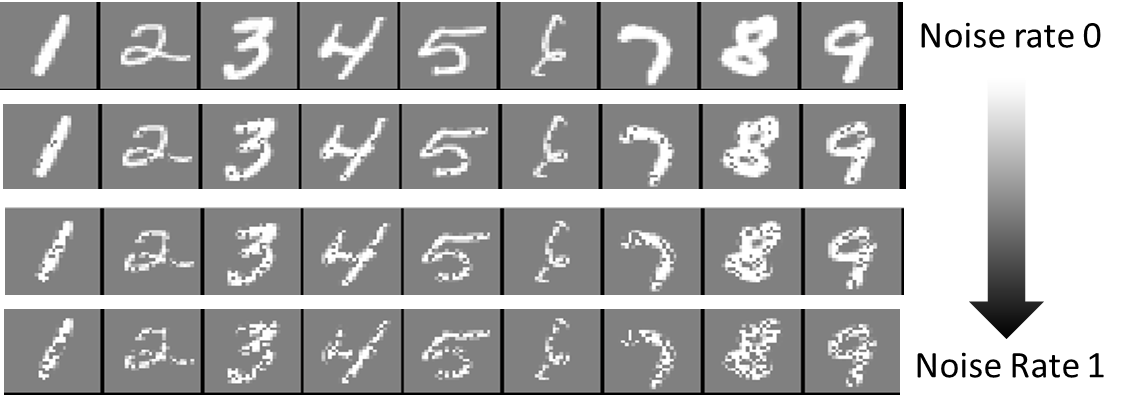
\includegraphics[scale=0.45]{fig/noise.png}
\caption{We add the noise (Salt \& Pepper niose) to the source data to generate the source domain with different relatedness to the target domain. From the images we  can see that the source domain is still related to the target domain in different level of the noise rate}\label{fig:noise}
\end{figure}

\subsection{Experiment result \& analysis}
\begin{table*}[htbp]
   \subfloat[Results on MNIST]{\resizebox{0.5\textwidth}{!}{
    \begin{tabular}{|c|c|c|c|c|c|c|c|}
     \hline 
      & \multicolumn{7}{c|}{Noise Level} \\ \hline
     & 0.0 & 0.2 & 0.3 & 0.5 & 0.8 & 0.9 & 1.0\\ \hline
      SMTLe\_s & \textbf{87.23} & \textbf{86.40} & \textbf{85.81} & \textbf{84.63} & \textbf{81.51} & \textbf{79.67} & \textbf{78.10}\\ 
      SMTLe\_m & 82.94 & 80.20 & 79.05 & 76.56 & 72.10 & 69.57 & 68.09\\ 
      MKT\_{m} & 61.96* & 57.14* & 55.18* & 50.67* & 45.16* & 43.72* & 42.73*\\ 
      MKT\_{s} & 86.63 & 82.33 & 79.78 & 74.61 & 67.51 & 65.52 & 64.06\\ 
      MKT\_{a} & 62.94 & 63.04 & 63.03 & 62.91 & 62.93 & 62.98 & 62.89\\ 
      MKTL & 70.06 & 55.63* & 60.42* & 41.57* & 40.44* & 42.22* & 31.44*\\ 
      PMT & 63.54 & 63.54 & 63.54 & 63.54 & 63.54 & 63.54 & 63.54\\ 
      Feature+ & 66.99 & 61.72* & 59.13* & 54.27* & 46.46* & 44.44* & 42.67*\\ 
      NT & 62.87 & 62.87 & 62.87 & 62.87 & 62.87 & 62.87 & 62.87\\ 
      Batch & 87.39 & 84.42 & 82.40 & 76.83 & 62.86* & 57.33* & 51.16*\\ 
\hline\end{tabular}}}%{body}
\subfloat[Results on USPS]{
    \resizebox{0.5\textwidth}{!}{
     \begin{tabular}{|c|c|c|c|c|c|c|c|}
          \hline 
          & \multicolumn{7}{c|}{Noise Level} \\ \hline
          & 0.0 & 0.2 & 0.3 & 0.5 & 0.8 & 0.9 & 1.0\\ \hline
           SMTLe\_s & \textbf{91.12} & 89.79 & 89.23 & 88.06 & 86.22 & 85.33 & 84.60\\ 
           SMTLe\_m & 90.78 & \textbf{89.85} & \textbf{89.42} & \textbf{88.55} & \textbf{86.80} & \textbf{85.96} & \textbf{84.91}\\ 
           MKT\_{m} & 86.80 & 84.80 & 83.57 & 81.02 & 75.96 & 74.53* & 72.73*\\ 
           MKT\_{s} & 64.18* & 61.39* & 61.80* & 62.93* & 64.85* & 65.29* & 65.55*\\ 
           MKT\_{a} & 75.76 & 75.76 & 75.75 & 75.79 & 75.75 & 75.78 & 75.84\\ 
           MKTL & 90.24 & 88.13 & 86.20 & 86.07 & 81.82 & 80.18 & 80.14\\ 
           PMT & 75.89 & 75.89 & 75.9 & 75.88 & 75.88 & 75.88 & 75.87\\ 
           Feature+ & 88.42 & 86.56 & 85.28 & 83.23 & 79.79 & 78.68 & 77.17\\ 
           NT & 75.75 & 75.75 & 75.75 & 75.75 & 75.75 & 75.75 & 75.75\\ 
           Batch & 91.65 & 90.38 & 89.58 & 87.36 & 82.55 & 80.52 & 77.84\\ 
     \hline\end{tabular}}}%
     \caption{Experiment results on 5 examples per class in target training set. We show the percentage of accuracy across the 10 classes on different noise level. We use "*" to denote the results suffer from negative transfer}\label{tab:rs}
  \end{table*}%
  
We perform the algorithms on different scenarios where the different level of noise is added to the source data to train the source models. Still we use LS-SVM to train the source models. For each dataset, we use the accuracy across the 10 classes as the criterion to evaluate the performance of the algorithms. We randomly split the original datasets into 3 sets and run 10 times to report the average performance. 

We show the performance of different algorithms on the two datasets under different noise level in Table \ref{tab:rs} where only 5 positive examples for each class are used in target training set. We show more results with different size of training examples in the target set in Table \ref{tab:mnist} and Table \ref{tab:usps}. From Table \ref{tab:rs} we can see that when there is no noise in the source data, most transfer algorithms can leverage the knowledge of the source model. Our methods $SMTLe_s$ and $SMTLe_m$ achieve the best performance among all transfer methods, but still slightly underperform the Batch method which can access all the data from both source and target training data. It is worthy to notice that the $MKT_m$ in MNIST and $MKT_s$ in USPS suffer from negative transfer even though there is no noise in the source data. This may cause by their weak regularization term which limits the transfer parameters within the ball with radium 1 (its default setting). The results could be improved if a better regularization can be found. As we add more noise into the source data, some of the transfer algorithms start to suffer from negative transfer. It is not surprising that all the methods (except for NT as no source knowledge is used) get a decreased performance. However, our methods can still outperform the other methods. The performance of MKTL in MNIST drops almost 39\%. MKTL tries to use aggressive augmentation approach and there are many parameters to learn. Therefore, it is more difficult to find the good solution when the source and target domain are not strongly related. In our method, We use simple feature augmentation approach. The optimal transfer parameters can both limit the VC dimension and reduce empirical risk at the same time. This promise that the target model can still perform well on the unseen data even though the source models become less related to the target domain. We can also see that there are just 3 methods that don't suffer from negative transfer in both datasets, i.e. $SMTLe_s$,$SMTLe_m$ and $MKT_a$. However, we can see that $MKT_a$ is a more conservative method which is reluctant to leverage the knowledge from the source model and as a result, it can successfully alleviate negative transfer and unable to fully exploit the knowledge from the source as well. 

In summary, in this section, we empirically evaluate the performance of our method in different scenarios where there is different relatedness between the source and target domains. Comparing with some baseline methods we can see that our method can effectively leverage the knowledge from the source models and alleviate negative transfer when other baseline methods suffer.

\begin{table*}[h]
\subfloat[10 examples per class]
{\resizebox{0.5\textwidth}{!}{\begin{tabular}{|c|c|c|c|c|c|c|c|}
     \hline 
     & \multicolumn{7}{c|}{Noise Level} \\ \hline
     & 0.0 & 0.2 & 0.3 & 0.5 & 0.8 & 0.9 & 1.0\\ \hline
      SMTLe\_s & \textbf{88.13} & \textbf{86.98} & \textbf{86.62} & \textbf{85.44} & \textbf{84.26} & \textbf{83.61} & \textbf{82.79}\\ 
      SMTLe\_m & 87.29 & 85.20 & 83.81 & 81.47 & 77.74 & 76.45 & 76.26\\ 
      MKT\_{m} & 65.01* & 61.51* & 59.02* & 53.92* & 49.24* & 48.34* & 47.51*\\ 
      MKT\_{s} & 87.82 & 85.88 & 84.00 & 80.85 & 75.87 & 73.81 & 72.30\\ 
      MKT\_{a} & 72.37 & 72.32 & 72.36 & 72.30 & 72.32 & 72.32 & 72.25\\ 
      MKTL & 79.63 & 68.80* & 69.55* & 59.74* & 52.04* & 50.47* & 42.47*\\ 
      Feature+ & 77.60 & 73.33 & 70.73* & 64.90* & 56.86* & 54.40* & 52.3*\\ 
      PMT & 72.86 & 72.87 & 72.87 & 72.87 & 72.86 & 72.86 & 72.87\\ 
      NT & 72.22 & 72.23 & 72.23 & 72.23 & 72.23 & 72.23 & 72.23\\ 
      Batch & 87.46 & 84.78 & 82.96 & 78.04 & 65.96* & 60.97* & 55.65*\\ 
\hline\end{tabular}}}\qquad
\subfloat[15 examples per class]{\resizebox{0.5\textwidth}{!}{\begin{tabular}{|c|c|c|c|c|c|c|c|}
     \hline 
     & \multicolumn{7}{c|}{Noise Level} \\ \hline
     & 0.0 & 0.2 & 0.3 & 0.5 & 0.8 & 0.9 & 1.0\\ \hline
      SMTLe\_s & 88.63 & \textbf{87.52} & \textbf{87.12} & \textbf{86.33} & \textbf{85.57} & \textbf{85.04} & \textbf{84.65}\\ 
      SMTLe\_m & \textbf{88.92} & 86.98 & 85.99 & 84.01 & 80.69 & 80.08 & 79.28\\ 
      MKT\_{m} & 67.03* & 63.34* & 61.31* & 56.26* & 51.76* & 50.72* & 49.69*\\ 
      MKT\_{s} & 88.08 & 86.31 & 85.40 & 83.38 & 79.52 & 77.83 & 77.04\\ 
      MKT\_{a} & 76.19 & 76.16 & 76.19 & 76.12 & 76.14 & 76.16 & 76.11\\ 
      MKTL & 83.75 & 74.27* & 77.46 & 66.39* & 61.57* & 60.0* & 55.28*\\ 
      Feature+ & 81.87 & 78.54 & 76.63 & 72.25* & 64.45* & 61.88* & 59.67*\\ 
      PMT & 76.78 & 76.78 & 76.78 & 76.79 & 76.78 & 76.78 & 76.78\\ 
      NT & 76.09 & 76.10 & 76.10 & 76.10 & 76.10 & 76.10 & 76.10\\ 
      Batch & 87.72 & 85.20 & 83.57 & 79.29 & 68.95* & 64.36* & 59.8*\\ 
\hline\end{tabular}}}\\
\subfloat[20 examples per class]{\resizebox{0.5\textwidth}{!}{\begin{tabular}{|c|c|c|c|c|c|c|c|}
     \hline 
     & \multicolumn{7}{c|}{Noise Level} \\ \hline
     & 0.0 & 0.2 & 0.3 & 0.5 & 0.8 & 0.9 & 1.0\\ \hline
      SMTLe\_s & 88.87 & 87.81 & \textbf{87.28} & \textbf{86.50} & \textbf{85.98} & \textbf{85.64} & \textbf{85.27}\\ 
      SMTLe\_m & \textbf{89.39} & \textbf{87.97} & 87.06 & 85.47 & 82.63 & 81.95 & 81.32\\ 
      MKT\_{m} & 68.03* & 64.37* & 62.7* & 58.98* & 54.41* & 53.52* & 52.93*\\ 
      MKT\_{s} & 88.04 & 86.42 & 85.58 & 83.69 & 81.29 & 80.66 & 79.56\\ 
      MKT\_{a} & 78.68 & 78.64 & 78.65 & 78.62 & 78.63 & 78.63 & 78.60\\ 
      MKTL & 86.75 & 81.14 & 82.46 & 72.57* & 65.4* & 69.53* & 61.56*\\ 
      Feature+ & 83.80 & 80.99 & 79.29 & 75.54* & 68.46* & 66.12* & 63.97*\\ 
      PMT & 78.43* & 78.43* & 78.44* & 78.44* & 78.43* & 78.43* & 78.43*\\ 
      NT & 78.58 & 78.59 & 78.59 & 78.60 & 78.60 & 78.59 & 78.60\\ 
      Batch & 87.80 & 85.41 & 83.89 & 80.10 & 71.22* & 67.35* & 63.28*\\ 
\hline\end{tabular}}}\qquad
\subfloat[25 examples per class]{\resizebox{0.5\textwidth}{!}{\begin{tabular}{|c|c|c|c|c|c|c|c|}
     \hline 
     & \multicolumn{7}{c|}{Noise Level} \\ \hline
     & 0.0 & 0.2 & 0.3 & 0.5 & 0.8 & 0.9 & 1.0\\ \hline
      SMTLe\_s & 89.22 & 88.16 & 87.67 & \textbf{86.94} & \textbf{86.46} & \textbf{86.26} & \textbf{85.95}\\ 
      SMTLe\_m & \textbf{89.69} & \textbf{88.7} & \textbf{87.72} & 86.33 & 83.95 & 83.23 & 82.73\\ 
      MKT\_{m} & 69.15* & 66.04* & 64.23* & 60.71* & 56.0* & 54.9* & 54.53*\\ 
      MKT\_{s} & 88.21 & 86.6 & 85.87 & 84.14 & 82.02 & 81.51 & 81.04\\ 
      MKT\_{a} & 80.35 & 80.33 & 80.36 & 80.33 & 80.33 & 80.33 & 80.31\\ 
      MKTL & 87.50 & 84.39 & 81.88 & 72.97* & 70.57* & 70.17* & 62.88*\\ 
      Feature+ & 85.23 & 82.76 & 81.21 & 77.66* & 71.59* & 69.39* & 67.48*\\ 
      PMT & 79.58* & 79.59* & 79.59* & 79.59* & 79.59* & 79.59* & 79.58*\\ 
      NT & 80.27 & 80.29 & 80.28 & 80.29 & 80.29 & 80.29 & 80.29\\ 
      Batch & 88.02 & 85.80 & 84.33 & 80.92 & 73.36* & 69.99* & 66.27*\\ 
\hline\end{tabular}}}\caption{Results on MNIST with 10/15/20/25 positive examples for each class}\label{tab:mnist}
\end{table*}



\begin{table*}
\subfloat[10 examples per class]{\resizebox{0.5\textwidth}{!}{\begin{tabular}{|c|c|c|c|c|c|c|c|}
     \hline 
     & \multicolumn{7}{c|}{Noise Level} \\ \hline
     & 0.0 & 0.2 & 0.3 & 0.5 & 0.8 & 0.9 & 1.0\\ \hline
      SMTLe\_s & \textbf{91.12} & 89.79 & 89.23 & 88.06 & 86.22 & 85.33 & 84.60\\ 
      SMTLe\_m & 90.78 & \textbf{89.85} & \textbf{89.42} & \textbf{88.55} & \textbf{86.80} & \textbf{85.96} & \textbf{84.91}\\ 
      MKT\_{m} & 86.80 & 84.80 & 83.57 & 81.02 & 75.96 & 74.53* & 72.73*\\ 
      MKT\_{s} & 64.18* & 61.39* & 61.80* & 62.93* & 64.85* & 65.29* & 65.55*\\ 
      MKT\_{a} & 75.76 & 75.76 & 75.75 & 75.79 & 75.75* & 75.78 & 75.84\\ 
      MKTL & 90.24 & 88.13 & 86.20 & 86.07 & 81.82 & 80.18 & 80.14\\ 
      Feature+ & 88.42 & 86.56 & 85.28 & 83.23 & 79.79 & 78.68 & 77.17\\ 
      PMT & 75.89 & 75.89 & 75.90 & 75.88 & 75.88 & 75.88 & 75.87\\ 
      NT & 75.75 & 75.75 & 75.74 & 75.76 & 75.76 & 75.76 & 75.74\\ 
      Batch & 91.65 & 90.38 & 89.58 & 87.36 & 82.55 & 80.52 & 77.84\\ 
\hline\end{tabular}}} \qquad
\subfloat[15 examples per class]{\resizebox{0.5\textwidth}{!}{\begin{tabular}{|c|c|c|c|c|c|c|c|}
     \hline 
     & \multicolumn{7}{c|}{Noise Level} \\ \hline
     & 0.0 & 0.2 & 0.3 & 0.5 & 0.8 & 0.9 & 1.0\\ \hline
      SMTLe\_s & \textbf{91.58} & 90.58 & 89.84 & 88.82 & 86.82 & 86.28 & 85.45\\ 
      SMTLe\_m & 91.46 & \textbf{90.72} & \textbf{90.29} & \textbf{89.61} & \textbf{88.22} & \textbf{87.89} & \textbf{87.19}\\ 
      MKT\_{m} & 89.06 & 87.98 & 87.31 & 85.46 & 81.94 & 80.29 & 78.51*\\ 
      MKT\_{s} & 74.12* & 71.44* & 71.63* & 72.16* & 73.36* & 73.56* & 73.56*\\ 
      MKT\_{a} & 79.57 & 79.57 & 79.55 & 79.58 & 79.57* & 79.59 & 79.58\\ 
      MKTL & 88.74 & 89.45 & 88.86 & 87.63 & 84.53 & 82.30 & 84.41\\ 
      Feature+ & 89.98 & 88.6 & 87.64 & 85.97 & 83.30 & 82.36 & 81.00\\ 
      PMT & 79.56 & 79.54* & 79.54 & 79.55* & 79.56* & 79.55* & 79.55\\ 
      NT & 79.55 & 79.56 & 79.54 & 79.57 & 79.57 & 79.58 & 79.54\\ 
      Batch & 91.75 & 90.61 & 89.88 & 88.04 & 84.25 & 82.69 & 80.80\\ 
\hline\end{tabular}}}\\
\subfloat[20 examples per class]{\resizebox{0.5\textwidth}{!}{\begin{tabular}{|c|c|c|c|c|c|c|c|}
     \hline 
     & \multicolumn{7}{c|}{Noise Level} \\ \hline
     & 0.0 & 0.2 & 0.3 & 0.5 & 0.8 & 0.9 & 1.0\\ \hline
      SMTLe\_s & 91.95 & 91.18 & 90.64 & 89.55 & 87.80 & 87.16 & 86.46\\ 
      SMTLe\_m & \textbf{92.01} & \textbf{91.25} & \textbf{90.79} & \textbf{90.20} & \textbf{89.03} & \textbf{88.70} & \textbf{88.30}\\ 
      MKT\_{m} & 89.90 & 89.05 & 88.64 & 87.12 & 82.78 & 81.21* & 79.44*\\ 
      MKT\_{s} & 79.39* & 76.88* & 76.84* & 77.31* & 78.02* & 78.13* & 78.03*\\ 
      MKT\_{a} & 81.92 & 81.92 & 81.92 & 81.93 & 81.94* & 81.94 & 81.91\\ 
      MKTL & 90.67 & 89.08 & 89.31 & 88.84 & 85.26 & 85.64 & 85.03\\ 
      Feature+ & 90.95 & 89.66 & 88.89 & 87.49 & 85.03 & 84.14 & 83.06\\ 
      PMT & 81.49* & 81.48* & 81.48* & 81.50* & 81.51* & 81.49* & 81.50*\\ 
      NT & 81.89 & 81.92 & 81.87 & 81.91 & 81.94 & 81.93 & 81.89\\ 
      Batch & 91.91 & 90.85 & 90.20 & 88.55 & 85.40 & 84.21 & 82.76\\ 
\hline\end{tabular}}}\qquad
\subfloat[25 examples per class]{\resizebox{0.5\textwidth}{!}{\begin{tabular}{|c|c|c|c|c|c|c|c|}
     \hline 
     & \multicolumn{7}{c|}{Noise Level} \\ \hline
     & 0.0 & 0.2 & 0.3 & 0.5 & 0.8 & 0.9 & 1.0\\ \hline
      SMTLe\_s & 92.18 & 91.43 & 90.93 & 89.97 & 88.41 & 87.83 & 87.22\\ 
      SMTLe\_m & \textbf{92.27} & \textbf{91.68} & \textbf{91.29} & \textbf{90.62} & \textbf{89.58} & \textbf{89.17} & \textbf{88.81}\\ 
      MKT\_{m} & 90.35 & 89.67 & 89.35 & 88.08 & 84.91 & 83.27* & 81.37*\\ 
      MKT\_{s} & 82.40* & 80.24* & 80.12* & 80.46* & 80.93* & 80.98* & 80.83*\\ 
      MKT\_{a} & 83.69 & 83.70 & 83.66 & 83.70 & 83.71 & 83.72 & 83.69\\ 
      MKTL & 91.55 & 90.46 & 90.01 & 88.49 & 87.36 & 86.47 & 87.02\\ 
      Feature+ & 91.38 & 90.26 & 89.56 & 88.38 & 86.42 & 85.63 & 84.67\\ 
      PMT & 82.89* & 82.87* & 82.88* & 82.88* & 82.89* & 82.88* & 82.9*\\ 
      NT & 83.66 & 83.69 & 83.65 & 83.68 & 83.71 & 83.70 & 83.65\\ 
      Batch & 92.11 & 91.08 & 90.50 & 89.06 & 86.34 & 85.30 & 84.27\\ 
\hline\end{tabular}}}\caption{Results on USPS with 10/15/20/25 positive examples for each class} \label{tab:usps}
\end{table*}



\section{Conclusion}
In this paper, we present a novel method called SMTLe that is able to transfer knowledge of the source model in domain adaptation. Inspired by previous work,
we propose a novel perspective on the work of HTL and show the reasons why positive and negative transfer would happen in the different scenario. Then based on our analysis, we propose our method SMTLe that can safely leverage the knowledge from the source models to achieve the improved performance of the target model by limiting the VC dimension of the transfer problem and reduce the empirical risk as well. Experiment results show that SMTLe can leverage related source knowledge and alleviate negative transfer in different scenarios and outperforms other baseline methods.

In our perspective on the domain adaptation problem, the data augmentation approach can fit a wider range of source classifiers. We can leverage the knowledge from any source model that can output the decision score/confidence, such as the Neural Networks and the inference model. There are still some problems to be solve while leveraging the source models with different kinds of classifiers how to better exploit the knowledge to both achieve good positive transfer performance and avoid negative transfer at the same time. This can be an important area in our future work.


% use section* for acknowledgment
\section*{Acknowledgment}


The authors would like to thank...

\appendices
\section{Convergence Analysis}\label{appd:convg}
\begin{theorem}
%Let $L(\beta)$ be a $\lambda$-strongly convex function in \eqref{eq:single:opti} and $\beta^*$ be its optimal solution.Let $\beta_1,...,\beta_{T+1}$ be a sequence such that $\beta_1 \in B$ and for $t>1$, we have $\beta_{t+1} = \beta_t - \eta_t \Delta_t$ , where $\Delta_t$ is the sub-gradient of $L(\beta_t)$ and $\eta_t = 1/(\lambda t)$. Assume we have $||\Delta_t|| \leq G$ for all $t$. Then we have:
	
	\begin{equation}
	L(\beta_{T+1}) \leq L(\beta^*)+\frac{G^2(1+\ln (T))}{2\lambda T}
	\end{equation}
\end{theorem}

\begin{proof}
	As $L(\beta)$ is strongly convex and $\Delta_t$ is in its sub-gradient set at $\beta_t$, according to the definition of $\lambda$-strong convexity \cite{rockafellar2015convex}, the following inequality holds:
	
	\begin{equation}\label{eq:app:strong}
		\left\langle {\beta_t - \beta^*,\Delta_t} \right\rangle \geq L(\beta_t)-L(\beta^*)+\frac{\lambda}{2}||\beta_t - \beta^*||^2
	\end{equation} 
	For the term $\left\langle {\beta_t - \beta^*,\Delta_y} \right\rangle$, it can be written as:
	
	\begin{equation} \label{eq:app:inner}
	\begin{aligned}
	\left\langle {\beta_t - \beta^*,\Delta_t} \right\rangle &= \left\langle {\beta_t - \frac{1}{2}\eta_t\Delta_t + \frac{1}{2}\eta_t\Delta_t- \beta^*,\Delta_t} \right\rangle\\
	&=\frac{1}{2}\left\langle {\left[ {\left( {{\beta _t} - {\eta _t}{\Delta _t}} \right) - {\beta ^*}} \right] + \left( {{\beta _t} - {\beta ^*}} \right) + {\eta _t}{\Delta _t},{\Delta _t}} \right\rangle \\
	&= \frac{1}{2}\left\langle {\left( {{\beta _{t + 1}} - {\beta ^*}} \right) + \left( {{\beta _t} - {\beta ^*}} \right),{\Delta _t}} \right\rangle  + \frac{1}{2}{\eta _t}\Delta _t^2\\
	&=\frac{1}{2}\left\langle {{\beta _{t + 1}} + {\beta _t} - 2{\beta ^*},{\Delta _t}} \right\rangle  + \frac{1}{2}{\eta _t}\Delta _t^2
	\end{aligned}
	\end{equation}
	
	Then we have:
	\begin{equation}\label{eq:app:squrediff}
	\begin{aligned}
	||\beta_t-\beta^*||^2-||\beta_{t+1}-\beta^*||^2 &= ( {{\beta _t} - {\beta _{t + 1}}})  ({{\beta _t} + {\beta _{t + 1}} - 2{\beta ^*}}) \\
	&=\left\langle {{\beta _{t + 1}} + {\beta _t} - 2{\beta ^*},{\eta_t\Delta _t}} \right\rangle
	\end{aligned}
	\end{equation}
	Using the assumption $||\Delta_t|| \leq G$, we can rearrange \eqref{eq:app:strong} and plug \eqref{eq:app:inner} and \eqref{eq:app:squrediff} into it, we have:
	
	\begin{equation}\label{eq:app:it_diff}
	\begin{aligned}
	&{Diff}_t = L(\beta_t)-L(\beta^*)\\
	 &\leq \frac{{||{\beta _t} - {\beta ^*}|{|^2} - ||{\beta _{t + 1}} - {\beta ^*}|{|^2}}}{{2{\eta _t}}} - \frac{\lambda }{2}||{\beta _t} - {\beta ^*}|{|^2} + \frac{1}{2}{\eta _t}\Delta _t^2 \\
	&\leq \frac{{||{\beta _t} - {\beta ^*}|{|^2} - ||{\beta _{t + 1}} - {\beta ^*}|{|^2}}}{{2{\eta _t}}} - \frac{\lambda }{2}||{\beta _t} - {\beta ^*}|{|^2} + \frac{1}{2}{\eta _t} G^2\\
	&=\frac{\lambda (t-1)}{2}{||{\beta _t} - {\beta ^*}||^2}- \frac{\lambda t}{2}{||{\beta _{t+1}} - {\beta ^*}||^2}+\frac{1}{2}{\eta _t} G^2
	\end{aligned}
	\end{equation}
	
	Due to the strong convexity, for each pair of $L(\beta_t)$ and $L(\beta_{t+1})$ for $t=1,...,T$, according to \eqref{eq:app:strong}, we have:
	
	\begin{equation}
	\begin{aligned}
	L({\beta _{t + 1}}) - L({\beta _t}) &\le \left\langle {{\beta _{t + 1}} - {\beta _t},{\Delta _t}} \right\rangle  - \frac{\lambda }{2}||{\beta _{t + 1}} - \beta_t |{|^2} \\
	&=  - \eta_t\Delta _t^2 (1-\frac{1}{2t}) \leq 0
	\end{aligned}
	\end{equation}
	Therefore, we have the following sequence $L(\beta^*) \leq L(\beta_T) \leq L(\beta_{T-1}) \leq...\leq L(\beta_1)$. 
	For the sequence $Diff_t$ for $t=1,...,T$, we have:
	
	\begin{equation} \label{eq:app:difsum}
	\sum_{t=1}^{T} Diff_t =  \sum_{t=1}^{T}L(\beta_t)-TL(\beta^*) \geq T\left[L(\beta_T)-L(\beta^*)\right]
	\end{equation}
	
	Next, we show that 
	
	\begin{equation}
	\begin{aligned}
	&\sum_{t=1}^{T} Diff_t =\\
	&\sum_{t=1}^{T}\left\{\frac{\lambda (t-1)}{2}{||{\beta _t} - {\beta ^*}||^2}- \frac{\lambda t}{2}{||{\beta _{t+1}} - {\beta ^*}||^2}+\frac{1}{2}{\eta _t} G^2\right\} \\
	&=-\frac{\lambda T}{2}{||{\beta _{T+1}-\beta^*}||^2} + \frac{G^2}{2 \lambda}\sum_{t=1}^{T} \frac{1}{t}\\
	&\leq \frac{G^2}{2 \lambda}\sum_{t=1}^{T} \frac{1}{t} \leq \frac{G^2}{2 \lambda}(1+\ln(T))
	\end{aligned}
	\end{equation}
	
	Combining \eqref{eq:app:difsum} and rearranging the result, we have:
	\begin{equation*}
	L(\beta_{T+1}) \leq L(\beta^*)+\frac{G^2(1+\ln (T))}{2\lambda T}
	\end{equation*}
\end{proof}

\section{Proof of avoiding negative transfer}\label{appd:proof}
%From the analysis in Appendix \ref{appd:convg} we can see that, SMITLe can alway converge to its optimal solution with sufficient iterations. We can prove that, with the optimal transfer parameters $\boldsymbol{\gamma}$ and $\boldsymbol{\beta}$, SMITLe can avoid negative transfer.

Assume that $\bar \xi_i$ is the multi-class loss of example $x_i$ without utilizing any prior knowledge, i.e. $\gamma=\beta = \mathbf{0}$. Let $\gamma^*, \beta^*$ be the optimal solution for Eq. \eqref{eq:dual} and $\xi_i^*$ be the multi-class loss with respective to example $x_i$. Then for every example $x_i \in \mathcal{X}$, we have:\[\sum\limits_i {{\xi^* _i}}  \le \sum\limits_i {{{\bar \xi }_i}} \]

\begin{proof}
%For simplification, let $\delta_i=1$ if $i=N+1$ and 0 otherwise, and  ${\theta _{ij}} = {\alpha ''_{ij}}\left( {1 - {\delta _j}} \right)/\psi_{ii}^{ - 1}$. Eq. \eqref{eq:train_loss} can be written as:
%\begin{equation}\label{eq:loss_simple}
%\begin{split}
%{\xi _i}(\gamma ,\beta )=&\mathop {\max }\limits_{n} \bigg \{ {\varepsilon _{n{y_i}}} - 1 + \frac{{\left( {{{\alpha '}_{i{y_i}}} - {{\alpha '}_{in}}} \right)}}{{\psi _{ii}^{ - 1}}} + {\theta _{in}}{\gamma _n} \\
%&- {\theta _{i{y_i}}}{\gamma _{{y_i}}} + \left( {{\delta _n} - {\delta _{{y_i}}}} \right)\sum\limits_k {\frac{{{{\alpha ''}_{ik}}{\beta _k}}}{{\psi_{ii}^{ - 1}}}}  \bigg\}
%\end{split}
%\end{equation}
When $\mathbf{\gamma}=\mathbf{\beta} = \mathbf{0}$, from Eq. \eqref{eq:train_loss} we can get:
\begin{equation*}
{\bar \xi _i} = \mathop {\max }\limits_n \left[ { {\varepsilon _{n{y_i}}}-1 + \frac{{\left( {{{\alpha '}_{i{y_i}}} - {{\alpha '}_{in}}} \right)}}{{\psi _{ii}^{ - 1}}}} \right]
\end{equation*}
%To obtain the optimal value of $\gamma$ and $\beta$, we have to seek the saddle point of the Lagrangian problem in \eqref{eq:dual} by finding the minimum for the prime variables $\left\{ \gamma, \beta, \xi \right\}$ and the maximum for the dual variables $\eta $.
For simplification, let $\delta_i=1$ if $i=N+1$ and 0 otherwise, and  ${\theta _{ij}} = {\alpha ''_{ij}}\left( {1 - {\delta _j}} \right)/\psi_{ii}^{ - 1}$.
To find the minimum of the primal problem, we require:
\begin{equation}
\frac{{\partial L}}{{\partial {\xi _i}}} = 1 - \sum\limits_n {{\eta _{in}}}  = 0 \Rightarrow \sum\limits_n {{\eta _{in}}}  = 1
\end{equation}   
%Similarly, for $\gamma$ and $\beta$, we require:
\begin{eqnarray}\label{eq:opt_gama}
\frac{{\partial L}}{{\partial {\gamma _n}}} = 0  
\Rightarrow  \gamma _n^* = \frac{1}{{{\lambda _1}}}\sum\limits_i {\left( {{\varepsilon _{n{y_i}}} - {\eta _{in}}} \right){\theta _{in}}} 
\end{eqnarray}
%In $=_1$ we use the facts that $\sum_n\eta_{in}=1$ and use $\varepsilon_{ny_i}$ to replace it.
\begin{eqnarray}\label{eq:opt_beta}
\frac{{\partial L}}{{\partial {\beta _n}}}  = 0 
\Rightarrow \beta _n^* = \frac{1}{{{\lambda _2}}}\sum\limits_{i,n} {\frac{{{\eta _{in}}{{\alpha ''}_{in}}}}{{\psi _{ii}^{ - 1}}}\left( {{\delta _{{y_i}}} - {\delta _n}} \right)} 
\end{eqnarray}
As the strong duality holds,the primal and dual objectives coincide. Plug Eq \eqref{eq:opt_gama} and \eqref{eq:opt_beta} into Eq. \eqref{eq:dual}, we have:
\begin{equation*}
\sum\limits_{i,n} {{\eta _{in}}\left[ {1 - {\varepsilon _{n{y_i}}} + {{\hat Y}_{in}}\left( {\gamma^* ,\beta^* } \right) - {{\hat Y}_{i{y_i}}}\left( {\gamma^* ,\beta^* } \right) - {\xi _i^*}} \right]}=0
\end{equation*}
Expand the equation above, we have:
\begin{eqnarray}\nonumber
\sum\limits_{i,n} {{\eta _{in}}\left[ { {\varepsilon _{n,{y_i}}}-1 + \frac{{\left( {{{\alpha '}_{i{y_i}}} - {{\alpha '}_{in}}} \right)}}{{\psi_{ii}^{ - 1}}} - {\xi _i}} \right]} \nonumber\\ 
= {\lambda _1}\sum\limits_r {{{\left\| {\gamma _r^*} \right\|}^2}}  + {\lambda _2}\sum\limits_r {{{\left\| {\beta _r^*} \right\|}^2}}  \ge 0\nonumber
\end{eqnarray}
Rearranging the above, we obtain:
\begin{eqnarray}\label{eq:link1}
\sum\limits_{i,n} {{\eta _{in}}\left[ { {\varepsilon _{n,{y_i}}} -1+ \frac{{\left( {{{\alpha '}_{i{y_i}}} - {{\alpha '}_{in}}} \right)}}{{\psi_{ii}^{ - 1}}}} \right]}  
 \ge \sum\limits_{i,n} {{\eta _{in}}{\xi _i}}  = \sum\limits_i {{\xi _i}} 
\end{eqnarray}
The left-hand side of Inequation \eqref{eq:link1} can be bounded by:
\begin{eqnarray}
&&\sum\limits_{i,n} {{\eta _{in}}\left[ { {\varepsilon _{n{y_i}}}-1 + \frac{{\left( {{{\alpha '}_{i{y_i}}} - {{\alpha '}_{in}}} \right)}}{{\psi_{ii}^{ - 1}}}} \right]} \nonumber\\ &&\le \sum\limits_i {\left( {\sum\limits_n {{\eta _{in}}\mathop {\max }\limits_r \left\{ { {\varepsilon _{r{y_i}}} -1 + \frac{{\left( {{{\alpha '}_{i{y_i}}} - {{\alpha '}_{ir}}} \right)}}{{\psi_{ii}^{ - 1}}}} \right\}} } \right)}  \nonumber\\
&&= \sum\limits_i {\left( {\sum\limits_n {{\eta _{in}}{{\bar \xi }_i}} } \right)}  = \sum\limits_i {\bar \xi_i }
\end{eqnarray}
\end{proof}

%\section{Results on MNIST and USPS}\label{appd:rs}
%\begin{table*}[h]
\subfloat[10 examples per class]
{\resizebox{0.5\textwidth}{!}{\begin{tabular}{|c|c|c|c|c|c|c|c|}
     \hline 
     & \multicolumn{7}{c|}{Noise Level} \\ \hline
     & 0.0 & 0.2 & 0.3 & 0.5 & 0.8 & 0.9 & 1.0\\ \hline
      SMTLe\_s & \textbf{88.13} & \textbf{86.98} & \textbf{86.62} & \textbf{85.44} & \textbf{84.26} & \textbf{83.61} & \textbf{82.79}\\ 
      SMTLe\_m & 87.29 & 85.20 & 83.81 & 81.47 & 77.74 & 76.45 & 76.26\\ 
      MKT\_{m} & 65.01* & 61.51* & 59.02* & 53.92* & 49.24* & 48.34* & 47.51*\\ 
      MKT\_{s} & 87.82 & 85.88 & 84.00 & 80.85 & 75.87 & 73.81 & 72.30\\ 
      MKT\_{a} & 72.37 & 72.32 & 72.36 & 72.30 & 72.32 & 72.32 & 72.25\\ 
      MKTL & 79.63 & 68.80* & 69.55* & 59.74* & 52.04* & 50.47* & 42.47*\\ 
      Feature+ & 77.60 & 73.33 & 70.73* & 64.90* & 56.86* & 54.40* & 52.3*\\ 
      PMT & 72.86 & 72.87 & 72.87 & 72.87 & 72.86 & 72.86 & 72.87\\ 
      NT & 72.22 & 72.23 & 72.23 & 72.23 & 72.23 & 72.23 & 72.23\\ 
      Batch & 87.46 & 84.78 & 82.96 & 78.04 & 65.96* & 60.97* & 55.65*\\ 
\hline\end{tabular}}}\qquad
\subfloat[15 examples per class]{\resizebox{0.5\textwidth}{!}{\begin{tabular}{|c|c|c|c|c|c|c|c|}
     \hline 
     & \multicolumn{7}{c|}{Noise Level} \\ \hline
     & 0.0 & 0.2 & 0.3 & 0.5 & 0.8 & 0.9 & 1.0\\ \hline
      SMTLe\_s & 88.63 & \textbf{87.52} & \textbf{87.12} & \textbf{86.33} & \textbf{85.57} & \textbf{85.04} & \textbf{84.65}\\ 
      SMTLe\_m & \textbf{88.92} & 86.98 & 85.99 & 84.01 & 80.69 & 80.08 & 79.28\\ 
      MKT\_{m} & 67.03* & 63.34* & 61.31* & 56.26* & 51.76* & 50.72* & 49.69*\\ 
      MKT\_{s} & 88.08 & 86.31 & 85.40 & 83.38 & 79.52 & 77.83 & 77.04\\ 
      MKT\_{a} & 76.19 & 76.16 & 76.19 & 76.12 & 76.14 & 76.16 & 76.11\\ 
      MKTL & 83.75 & 74.27* & 77.46 & 66.39* & 61.57* & 60.0* & 55.28*\\ 
      Feature+ & 81.87 & 78.54 & 76.63 & 72.25* & 64.45* & 61.88* & 59.67*\\ 
      PMT & 76.78 & 76.78 & 76.78 & 76.79 & 76.78 & 76.78 & 76.78\\ 
      NT & 76.09 & 76.10 & 76.10 & 76.10 & 76.10 & 76.10 & 76.10\\ 
      Batch & 87.72 & 85.20 & 83.57 & 79.29 & 68.95* & 64.36* & 59.8*\\ 
\hline\end{tabular}}}\\
\subfloat[20 examples per class]{\resizebox{0.5\textwidth}{!}{\begin{tabular}{|c|c|c|c|c|c|c|c|}
     \hline 
     & \multicolumn{7}{c|}{Noise Level} \\ \hline
     & 0.0 & 0.2 & 0.3 & 0.5 & 0.8 & 0.9 & 1.0\\ \hline
      SMTLe\_s & 88.87 & 87.81 & \textbf{87.28} & \textbf{86.50} & \textbf{85.98} & \textbf{85.64} & \textbf{85.27}\\ 
      SMTLe\_m & \textbf{89.39} & \textbf{87.97} & 87.06 & 85.47 & 82.63 & 81.95 & 81.32\\ 
      MKT\_{m} & 68.03* & 64.37* & 62.7* & 58.98* & 54.41* & 53.52* & 52.93*\\ 
      MKT\_{s} & 88.04 & 86.42 & 85.58 & 83.69 & 81.29 & 80.66 & 79.56\\ 
      MKT\_{a} & 78.68 & 78.64 & 78.65 & 78.62 & 78.63 & 78.63 & 78.60\\ 
      MKTL & 86.75 & 81.14 & 82.46 & 72.57* & 65.4* & 69.53* & 61.56*\\ 
      Feature+ & 83.80 & 80.99 & 79.29 & 75.54* & 68.46* & 66.12* & 63.97*\\ 
      PMT & 78.43* & 78.43* & 78.44* & 78.44* & 78.43* & 78.43* & 78.43*\\ 
      NT & 78.58 & 78.59 & 78.59 & 78.60 & 78.60 & 78.59 & 78.60\\ 
      Batch & 87.80 & 85.41 & 83.89 & 80.10 & 71.22* & 67.35* & 63.28*\\ 
\hline\end{tabular}}}\qquad
\subfloat[25 examples per class]{\resizebox{0.5\textwidth}{!}{\begin{tabular}{|c|c|c|c|c|c|c|c|}
     \hline 
     & \multicolumn{7}{c|}{Noise Level} \\ \hline
     & 0.0 & 0.2 & 0.3 & 0.5 & 0.8 & 0.9 & 1.0\\ \hline
      SMTLe\_s & 89.22 & 88.16 & 87.67 & \textbf{86.94} & \textbf{86.46} & \textbf{86.26} & \textbf{85.95}\\ 
      SMTLe\_m & \textbf{89.69} & \textbf{88.7} & \textbf{87.72} & 86.33 & 83.95 & 83.23 & 82.73\\ 
      MKT\_{m} & 69.15* & 66.04* & 64.23* & 60.71* & 56.0* & 54.9* & 54.53*\\ 
      MKT\_{s} & 88.21 & 86.6 & 85.87 & 84.14 & 82.02 & 81.51 & 81.04\\ 
      MKT\_{a} & 80.35 & 80.33 & 80.36 & 80.33 & 80.33 & 80.33 & 80.31\\ 
      MKTL & 87.50 & 84.39 & 81.88 & 72.97* & 70.57* & 70.17* & 62.88*\\ 
      Feature+ & 85.23 & 82.76 & 81.21 & 77.66* & 71.59* & 69.39* & 67.48*\\ 
      PMT & 79.58* & 79.59* & 79.59* & 79.59* & 79.59* & 79.59* & 79.58*\\ 
      NT & 80.27 & 80.29 & 80.28 & 80.29 & 80.29 & 80.29 & 80.29\\ 
      Batch & 88.02 & 85.80 & 84.33 & 80.92 & 73.36* & 69.99* & 66.27*\\ 
\hline\end{tabular}}}\caption{Results on MNIST with 10/15/20/25 positive examples for each class}\label{tab:mnist}
\end{table*}



\begin{table*}
\subfloat[10 examples per class]{\resizebox{0.5\textwidth}{!}{\begin{tabular}{|c|c|c|c|c|c|c|c|}
     \hline 
     & \multicolumn{7}{c|}{Noise Level} \\ \hline
     & 0.0 & 0.2 & 0.3 & 0.5 & 0.8 & 0.9 & 1.0\\ \hline
      SMTLe\_s & \textbf{91.12} & 89.79 & 89.23 & 88.06 & 86.22 & 85.33 & 84.60\\ 
      SMTLe\_m & 90.78 & \textbf{89.85} & \textbf{89.42} & \textbf{88.55} & \textbf{86.80} & \textbf{85.96} & \textbf{84.91}\\ 
      MKT\_{m} & 86.80 & 84.80 & 83.57 & 81.02 & 75.96 & 74.53* & 72.73*\\ 
      MKT\_{s} & 64.18* & 61.39* & 61.80* & 62.93* & 64.85* & 65.29* & 65.55*\\ 
      MKT\_{a} & 75.76 & 75.76 & 75.75 & 75.79 & 75.75* & 75.78 & 75.84\\ 
      MKTL & 90.24 & 88.13 & 86.20 & 86.07 & 81.82 & 80.18 & 80.14\\ 
      Feature+ & 88.42 & 86.56 & 85.28 & 83.23 & 79.79 & 78.68 & 77.17\\ 
      PMT & 75.89 & 75.89 & 75.90 & 75.88 & 75.88 & 75.88 & 75.87\\ 
      NT & 75.75 & 75.75 & 75.74 & 75.76 & 75.76 & 75.76 & 75.74\\ 
      Batch & 91.65 & 90.38 & 89.58 & 87.36 & 82.55 & 80.52 & 77.84\\ 
\hline\end{tabular}}} \qquad
\subfloat[15 examples per class]{\resizebox{0.5\textwidth}{!}{\begin{tabular}{|c|c|c|c|c|c|c|c|}
     \hline 
     & \multicolumn{7}{c|}{Noise Level} \\ \hline
     & 0.0 & 0.2 & 0.3 & 0.5 & 0.8 & 0.9 & 1.0\\ \hline
      SMTLe\_s & \textbf{91.58} & 90.58 & 89.84 & 88.82 & 86.82 & 86.28 & 85.45\\ 
      SMTLe\_m & 91.46 & \textbf{90.72} & \textbf{90.29} & \textbf{89.61} & \textbf{88.22} & \textbf{87.89} & \textbf{87.19}\\ 
      MKT\_{m} & 89.06 & 87.98 & 87.31 & 85.46 & 81.94 & 80.29 & 78.51*\\ 
      MKT\_{s} & 74.12* & 71.44* & 71.63* & 72.16* & 73.36* & 73.56* & 73.56*\\ 
      MKT\_{a} & 79.57 & 79.57 & 79.55 & 79.58 & 79.57* & 79.59 & 79.58\\ 
      MKTL & 88.74 & 89.45 & 88.86 & 87.63 & 84.53 & 82.30 & 84.41\\ 
      Feature+ & 89.98 & 88.6 & 87.64 & 85.97 & 83.30 & 82.36 & 81.00\\ 
      PMT & 79.56 & 79.54* & 79.54 & 79.55* & 79.56* & 79.55* & 79.55\\ 
      NT & 79.55 & 79.56 & 79.54 & 79.57 & 79.57 & 79.58 & 79.54\\ 
      Batch & 91.75 & 90.61 & 89.88 & 88.04 & 84.25 & 82.69 & 80.80\\ 
\hline\end{tabular}}}\\
\subfloat[20 examples per class]{\resizebox{0.5\textwidth}{!}{\begin{tabular}{|c|c|c|c|c|c|c|c|}
     \hline 
     & \multicolumn{7}{c|}{Noise Level} \\ \hline
     & 0.0 & 0.2 & 0.3 & 0.5 & 0.8 & 0.9 & 1.0\\ \hline
      SMTLe\_s & 91.95 & 91.18 & 90.64 & 89.55 & 87.80 & 87.16 & 86.46\\ 
      SMTLe\_m & \textbf{92.01} & \textbf{91.25} & \textbf{90.79} & \textbf{90.20} & \textbf{89.03} & \textbf{88.70} & \textbf{88.30}\\ 
      MKT\_{m} & 89.90 & 89.05 & 88.64 & 87.12 & 82.78 & 81.21* & 79.44*\\ 
      MKT\_{s} & 79.39* & 76.88* & 76.84* & 77.31* & 78.02* & 78.13* & 78.03*\\ 
      MKT\_{a} & 81.92 & 81.92 & 81.92 & 81.93 & 81.94* & 81.94 & 81.91\\ 
      MKTL & 90.67 & 89.08 & 89.31 & 88.84 & 85.26 & 85.64 & 85.03\\ 
      Feature+ & 90.95 & 89.66 & 88.89 & 87.49 & 85.03 & 84.14 & 83.06\\ 
      PMT & 81.49* & 81.48* & 81.48* & 81.50* & 81.51* & 81.49* & 81.50*\\ 
      NT & 81.89 & 81.92 & 81.87 & 81.91 & 81.94 & 81.93 & 81.89\\ 
      Batch & 91.91 & 90.85 & 90.20 & 88.55 & 85.40 & 84.21 & 82.76\\ 
\hline\end{tabular}}}\qquad
\subfloat[25 examples per class]{\resizebox{0.5\textwidth}{!}{\begin{tabular}{|c|c|c|c|c|c|c|c|}
     \hline 
     & \multicolumn{7}{c|}{Noise Level} \\ \hline
     & 0.0 & 0.2 & 0.3 & 0.5 & 0.8 & 0.9 & 1.0\\ \hline
      SMTLe\_s & 92.18 & 91.43 & 90.93 & 89.97 & 88.41 & 87.83 & 87.22\\ 
      SMTLe\_m & \textbf{92.27} & \textbf{91.68} & \textbf{91.29} & \textbf{90.62} & \textbf{89.58} & \textbf{89.17} & \textbf{88.81}\\ 
      MKT\_{m} & 90.35 & 89.67 & 89.35 & 88.08 & 84.91 & 83.27* & 81.37*\\ 
      MKT\_{s} & 82.40* & 80.24* & 80.12* & 80.46* & 80.93* & 80.98* & 80.83*\\ 
      MKT\_{a} & 83.69 & 83.70 & 83.66 & 83.70 & 83.71 & 83.72 & 83.69\\ 
      MKTL & 91.55 & 90.46 & 90.01 & 88.49 & 87.36 & 86.47 & 87.02\\ 
      Feature+ & 91.38 & 90.26 & 89.56 & 88.38 & 86.42 & 85.63 & 84.67\\ 
      PMT & 82.89* & 82.87* & 82.88* & 82.88* & 82.89* & 82.88* & 82.9*\\ 
      NT & 83.66 & 83.69 & 83.65 & 83.68 & 83.71 & 83.70 & 83.65\\ 
      Batch & 92.11 & 91.08 & 90.50 & 89.06 & 86.34 & 85.30 & 84.27\\ 
\hline\end{tabular}}}\caption{Results on USPS with 10/15/20/25 positive examples for each class} \label{tab:usps}
\end{table*}



\bibliographystyle{IEEEtran}
\bibliography{research}


% An example of a floating figure using the graphicx package.
% Note that \label must occur AFTER (or within) \caption.
% For figures, \caption should occur after the \includegraphics.
% Note that IEEEtran v1.7 and later has special internal code that
% is designed to preserve the operation of \label within \caption
% even when the captionsoff option is in effect. However, because
% of issues like this, it may be the safest practice to put all your
% \label just after \caption rather than within \caption{}.
%
% Reminder: the "draftcls" or "draftclsnofoot", not "draft", class
% option should be used if it is desired that the figures are to be
% displayed while in draft mode.
%
%\begin{figure}[!t]
%\centering
%\includegraphics[width=2.5in]{myfigure}
% where an .eps filename suffix will be assumed under latex,
% and a .pdf suffix will be assumed for pdflatex; or what has been declared
% via \DeclareGraphicsExtensions.
%\caption{Simulation results for the network.}
%\label{fig_sim}
%\end{figure}

% Note that the IEEE typically puts floats only at the top, even when this
% results in a large percentage of a column being occupied by floats.


% An example of a double column floating figure using two subfigures.
% (The subfig.sty package must be loaded for this to work.)
% The subfigure \label commands are set within each subfloat command,
% and the \label for the overall figure must come after \caption.
% \hfil is used as a separator to get equal spacing.
% Watch out that the combined width of all the subfigures on a
% line do not exceed the text width or a line break will occur.
%
%\begin{figure*}[!t]
%\centering
%\subfloat[Case I]{\includegraphics[width=2.5in]{box}%
%\label{fig_first_case}}
%\hfil
%\subfloat[Case II]{\includegraphics[width=2.5in]{box}%
%\label{fig_second_case}}
%\caption{Simulation results for the network.}
%\label{fig_sim}
%\end{figure*}
%
% Note that often IEEE papers with subfigures do not employ subfigure
% captions (using the optional argument to \subfloat[]), but instead will
% reference/describe all of them (a), (b), etc., within the main caption.
% Be aware that for subfig.sty to generate the (a), (b), etc., subfigure
% labels, the optional argument to \subfloat must be present. If a
% subcaption is not desired, just leave its contents blank,
% e.g., \subfloat[].


% An example of a floating table. Note that, for IEEE style tables, the
% \caption command should come BEFORE the table and, given that table
% captions serve much like titles, are usually capitalized except for words
% such as a, an, and, as, at, but, by, for, in, nor, of, on, or, the, to
% and up, which are usually not capitalized unless they are the first or
% last word of the caption. Table text will default to \footnotesize as
% the IEEE normally uses this smaller font for tables.
% The \label must come after \caption as always.
%
%\begin{table}[!t]
%% increase table row spacing, adjust to taste
%\renewcommand{\arraystretch}{1.3}
% if using array.sty, it might be a good idea to tweak the value of
% \extrarowheight as needed to properly center the text within the cells
%\caption{An Example of a Table}
%\label{table_example}
%\centering
%% Some packages, such as MDW tools, offer better commands for making tables
%% than the plain LaTeX2e tabular which is used here.
%\begin{tabular}{|c||c|}
%\hline
%One & Two\\
%\hline
%Three & Four\\
%\hline
%\end{tabular}
%\end{table}


% Note that the IEEE does not put floats in the very first column
% - or typically anywhere on the first page for that matter. Also,
% in-text middle ("here") positioning is typically not used, but it
% is allowed and encouraged for Computer Society conferences (but
% not Computer Society journals). Most IEEE journals/conferences use
% top floats exclusively.
% Note that, LaTeX2e, unlike IEEE journals/conferences, places
% footnotes above bottom floats. This can be corrected via the
% \fnbelowfloat command of the stfloats package.





% conference papers do not normally have an appendix








% trigger a \newpage just before the given reference
% number - used to balance the columns on the last page
% adjust value as needed - may need to be readjusted if
% the document is modified later
%\IEEEtriggeratref{8}
% The "triggered" command can be changed if desired:
%\IEEEtriggercmd{\enlargethispage{-5in}}

% references section

% can use a bibliography generated by BibTeX as a .bbl file
% BibTeX documentation can be easily obtained at:
% http://mirror.ctan.org/biblio/bibtex/contrib/doc/
% The IEEEtran BibTeX style support page is at:
% http://www.michaelshell.org/tex/ieeetran/bibtex/
%\bibliographystyle{IEEEtran}
% argument is your BibTeX string definitions and bibliography database(s)
%\bibliography{IEEEabrv,../bib/paper}
%
% <OR> manually copy in the resultant .bbl file
% set second argument of \begin to the number of references
% (used to reserve space for the reference number labels box)




% that's all folks
\end{document}


